\documentclass[11pt,a4paper]{article}
% =====================================================================
% PLOS NTD revision v18 (submission-clean candidate).
% PROVENANCE: Derived directly from the preserved revision v17 (exact-wording
% verification) source. v18 is a manuscript-cleaning and submission-preparation pass
% only: NO scientific number, model, prediction, interval, threshold, horizon, regime or
% sensitivity was rerun or changed. It removes internal workflow wording from the
% public-facing text (title-page internal notice box and internal filenames),
% corrects the Author Summary and AI-assistance wording, and neutralizes Supporting-
% Information status labels. Internal metadata/QC records are kept only under
% internal_review_only/. The submission metadata gate is tracked in
% submission_metadata_gate_v18.md (not referenced in the manuscript body).
% Two build modes (first-page notice only): default = scientifically-cleaned author-review
% copy (metadata/declarations incomplete); \internalcompletion = internal author-completion
% copy. No submission-ready PDF is produced while mandatory gate items remain OPEN.
% =====================================================================
\usepackage[utf8]{inputenc}
\usepackage[T1]{fontenc}
\usepackage{lmodern}
\usepackage{amsmath,amsfonts,amssymb}
\usepackage{booktabs}
\usepackage{graphicx}
\usepackage{threeparttable}
\usepackage{geometry}
\usepackage{microtype}
\usepackage{tabularx}
\usepackage{array}
\usepackage{float}
\usepackage{placeins}
\usepackage{pgfplots}
\pgfplotsset{compat=1.18}
% Force fixed-point (non-scientific) y-axis tick labels on all plots.
\pgfplotsset{every axis/.append style={scaled y ticks=false, yticklabel style={/pgf/number format/.cd, fixed, precision=2, /tikz/.cd}}}
\usepackage{tikz}
\usepackage{xcolor}
\usepackage{setspace}
\usepackage[numbers,sort&compress]{natbib}
\usepackage[colorlinks=true,linkcolor=black,citecolor=black,urlcolor=black]{hyperref}
\usepackage{lineno}
\usetikzlibrary{arrows.meta, positioning, shapes.geometric, patterns}

% ---- Okabe-Ito colorblind-safe palette (grayscale-legible) ----
\definecolor{okBlue}{RGB}{0,114,178}
\definecolor{okOrange}{RGB}{230,159,0}
\definecolor{okGreen}{RGB}{0,158,115}
\definecolor{okVermillion}{RGB}{213,94,0}
\definecolor{okPurple}{RGB}{204,121,167}
\definecolor{okSky}{RGB}{86,180,233}
\definecolor{okYellow}{RGB}{240,228,66}
\definecolor{okGray}{RGB}{120,120,120}

\geometry{margin=1in}
\usepackage{fancyhdr}
\pagestyle{fancy}\fancyhf{}
\fancyhead[R]{\scriptsize Climate-informed dengue warning beyond surveillance}
\fancyfoot[R]{\footnotesize\thepage}
\renewcommand{\headrulewidth}{0pt}
\doublespacing
% Line numbers OFF by default (author standing preference for review/reading copies).
% The line-numbered review build defines \linenumberedcopy on the command line to enable
% them without editing this file (PLOS submission build should also enable them).
\ifdefined\linenumberedcopy \linenumbers \fi

\begin{document}

% =====================================================================
% TITLE PAGE
% =====================================================================
\thispagestyle{fancy}
\begin{center}
{\Large \textbf{Standard evaluation can overstate the incremental value of climate data for dengue alerting: a surveillance-benchmarked, matched-baseline decision-curve reanalysis in Sri Lanka and Colombia}}\\[1.0em]

{\normalsize \textbf{Short title:} Matched-baseline evaluation of climate value for dengue alerting}\\[1.2em]

Ganesh Shiwakoti\textsuperscript{1,\,$\ast$}, Bhimsen Khadka\textsuperscript{2}, and Ajay Kumar Thapa\textsuperscript{3}\\[0.6em]

\footnotesize
\textsuperscript{1}Department of Mathematics and Statistics, Florida Atlantic University, Boca Raton, Florida, USA\\
\textsuperscript{2}Department of Mathematical Sciences, The University of Texas at Dallas, Richardson, Texas, USA\\
\textsuperscript{3}Department of Civil, Environmental and Geomatics Engineering, Florida Atlantic University, Boca Raton, Florida, USA\\[0.3em]
$\ast$\,Corresponding author: ganshiwakoti@gmail.com
\end{center}

\vspace{1em}
\begin{center}
\ifdefined\internalcompletion
\fbox{\parbox{0.85\linewidth}{\centering\footnotesize \textbf{Internal author-completion copy.} Author metadata and declarations---coauthor emails, ORCIDs, CRediT contributions, author-order and manuscript approval, accountability confirmation, ethics determination, funding, competing interests, acknowledgments, repository URL, code and derived-data licensing, archival identifier, OpenDengue access-date, AI-disclosure approval, and completion of Supporting-Information checklists---remain to be confirmed by the authors before submission.}}
\else
\fbox{\parbox{0.85\linewidth}{\centering\footnotesize Scientifically cleaned author-review copy. Submission metadata and declarations remain incomplete.}}
\fi
\end{center}

\newpage

% =====================================================================
% STRUCTURED ABSTRACT (PLOS NTD: Background / Methodology & Principal
% Findings / Conclusions & Significance; 250-300 words; NO citations)
% =====================================================================
\begin{abstract}
\noindent\textbf{Background.}
Climate-informed dengue early-warning systems are usually judged by discrimination (the area under the receiver-operating characteristic curve) and against less demanding comparators such as seasonal climatology. Public-health deployment, however, depends on whether predicted risks improve calibrated, threshold-based alert decisions beyond the information already available from routine surveillance.

\noindent\textbf{Methodology/Principal Findings.}
We conducted a retrospective decision-evaluation for short-horizon elevated-activity alerting in Sri Lanka (primary, RDHS-week, 2018--2025) and Colombia (a second, differently-constructed case study using a selected common-complete municipality subset, 2020--2022), comparing a recent-case surveillance baseline (M1) with climate-only and hybrid models by calibration, recalibration, and decision-curve net benefit ($h=4$, reference threshold $p^*=0.30$). Recent surveillance was a demanding benchmark: climate-only models added no incremental decision value beyond recent surveillance, and the pre-specified primary hybrid contrast in Sri Lanka was null ($\Delta$NB(M4$-$M1) $=-0.008$, 95\% CI $-0.028$ to $+0.013$). This null was calibration-sensitive: the primary contrasts used raw predictions, and an out-of-fold internal recalibration (an optimistic cross-fit using concurrent test-period weeks, not a past-only operational procedure) moved $\Delta$NB(M4$-$M1) to $+0.009$ (95\% CI including zero), so neither raw nor recalibrated contrasts established a hybrid benefit. In Colombia the full hybrid exceeded M1 by $+0.0188$, but M5 adds seasonal terms and department fixed effects M1 lacks; matching that structure reduced the climate increment to $+0.0078$ (95\% CI $+0.0039$ to $+0.0119$), about half the compound difference. This small increment did not grow with lead time and attenuated toward zero under a reporting-delay sensitivity (three-week matched $+0.0049$); its robustness to period could not be established, and it did not appear in Sri Lanka. The two settings used differently constructed exposures (humidity in Sri Lanka only) and were not formally compared.

\noindent\textbf{Conclusions/Significance.}
Evaluations that benchmark climate against weak comparators or leave non-climate structure unmatched can overstate the decision value of climate data for dengue alerting. Benchmarked against recent surveillance, matched for structure, and judged by calibrated decision-curve net benefit, climate added little robust standalone value: Sri Lanka was null (and calibration-sensitive) and the small Colombia matched increment did not survive as robust, transportable evidence. The contribution is primarily methodological---benchmark against recent surveillance, match non-climate structure before attributing value to climate, and report calibration and threshold-averaged net benefit rather than discrimination against weak comparators. Local, setting-specific evaluation remains necessary.
\end{abstract}

% =====================================================================
% AUTHOR SUMMARY (150-200 words; nontechnical; first-person; no acronyms)
% =====================================================================
\section*{Author Summary}
Dengue early-warning systems often use weather and climate data to anticipate weeks of elevated dengue activity, but health agencies already track recent case counts, which carry strong short-term information. We asked whether adding climate improves alert decisions beyond what recent cases already show. In Sri Lanka and Colombia we compared models against a recent-surveillance benchmark, judging them by how well their predicted risks support real alert decisions, not only by ranking accuracy. Recent surveillance was hard to beat, and climate-only models added little. In Sri Lanka the originally planned combined model did not clearly improve on surveillance, and this result was sensitive to how the models' probabilities were calibrated. In Colombia the combined model looked better, but it also included seasonal and location terms the surveillance model lacked; after matching those, only a small climate improvement remained, and it did not grow at longer lead times and weakened under a surveillance-lag feature-censoring sensitivity intended to mimic reporting delay. Because the two countries were studied differently, each result needs local interpretation. Our main message concerns evaluation: judging climate models against weak baselines, or without matching this extra structure, can yield a larger estimated value for climate than a structure-matched surveillance comparison.

% =====================================================================
% INTRODUCTION
% =====================================================================
\section{Introduction}

Dengue is a major public-health challenge across tropical and subtropical regions, and early-warning systems are widely promoted to anticipate periods of elevated transmission. Transmission depends on mosquito ecology, human susceptibility, movement, public-health control, and environmental conditions, and climate variables such as temperature, humidity, and rainfall influence mosquito abundance, survival, biting, and viral replication, which makes climate-informed early warning conceptually attractive~\cite{Mordecai2017,Huber2018}.

Most dengue early-warning studies evaluate prediction models using discrimination or forecast-accuracy metrics~\cite{Johansson2019,Baharom2022,HussainAlkhateeb2021,Lowe2021}. Discrimination describes whether a model ranks high-risk periods above low-risk periods, but it is incomplete for operational decision-making. A public-health alert system must support threshold-based action, and a model with acceptable discrimination may still be poorly calibrated or may fail to improve net benefit relative to simpler alert strategies. Calibration is therefore central, because decisions depend on predicted probabilities and because calibration can drift when the deployment period differs in baseline incidence from the training period~\cite{VanCalster2019,VanCalster2023,SteyerbergVergouwe2014}.

Decision-curve analysis offers a complementary evaluation of whether a model improves threshold-based decisions~\cite{Vickers2006,Vickers2016,Vickers2019}. Net benefit weighs true-positive gains against the false-positive cost implied by a decision threshold, which connects to cost--loss reasoning in which the threshold encodes the trade-off between unnecessary response and missed elevated transmission~\cite{Murphy1985,Tozan2023}. The relevant comparison, however, is frequently overlooked. A central and demanding benchmark is recent dengue surveillance itself: because incidence is temporally autocorrelated, recent case counts contain strong short-term information, and a climate-informed model that appears useful against a climatological or null baseline may add little beyond information agencies already hold. Health agencies already hold recent case counts, which carry strong short-term information; prominent deployed early-warning systems such as EWARS-csd are, by contrast, \emph{climate}-driven (a distributed-lag nonlinear model of temperature and rainfall within a Bayesian INLA framework, validated by sensitivity and predictive value across endemicity in Colombian municipalities---the same country as our secondary setting) rather than benchmarked against a recent-case model or evaluated by decision-curve net benefit~\cite{EWARScsd}---the evaluation gap this study addresses.

The operational question is therefore not whether climate carries predictive signal for dengue beyond chance, but whether climate adds value beyond recent cases, and whether any such value is visible under calibration and decision-curve evaluation rather than discrimination alone. We address this question with a surveillance-benchmarked, calibration-aware, decision-analytic framework. The primary analysis uses Sri Lanka RDHS-week surveillance linked to climate and population data, with a date-aligned linkage between weekly reports and ISO climate weeks. We apply the same evaluation logic to Colombia as a second, differently-constructed case study, refitting all models locally rather than transporting coefficients, to assess whether locally refitted climate-only or climate--surveillance hybrid models add calibrated decision value beyond recent surveillance. That recent-case autocorrelation can dominate climate for short-term dengue prediction has been reported before: in Mexico, climate data did not significantly improve seasonal autoregressive forecasts under out-of-sample evaluation~\cite{Johansson2016}. Yet dengue early-warning models remain predominantly climate-driven and are typically judged by discrimination against weak comparators, with external validation and calibration rarely reported~\cite{Leung2022,HussainAlkhateeb2021}. Our contribution is therefore not a new forecasting model, nor a new empirical claim that climate is weak, but an evaluation framework for climate-informed dengue alerting: benchmarking against a recent-case surveillance model, judging by calibration and decision-curve net benefit rather than discrimination, and---critically---using a specification-matched baseline to separate any climate contribution from non-climate seasonal and geographic structure. Benchmarking a dengue early-warning model against a model mirroring current surveillance is not itself new~\cite{Lowe2013}, and weather-only models have been found to add no practical advantage over surveillance data~\cite{Benedum2020}; our recent-case baseline (M1) is a stronger autoregressive comparator, and the empirical result is confirmatory. We do not claim methodological novelty for calibration or decision-curve analysis themselves---both have recently been applied to dengue prognosis~\cite{Sangkaew2026}; the genuinely novel piece is the matched-baseline attribution separating any climate contribution from seasonal and geographic structure.

% =====================================================================
% METHODS
% =====================================================================
\section{Methods}

\subsection{Study design and reporting}
We conducted a retrospective decision-evaluation of dengue early-warning models using weekly surveillance, climate, population, and spatial data. The aim was not to develop a forecasting model but to evaluate whether climate-informed models add operational decision value beyond recent dengue surveillance, judged by discrimination, calibration, time-updated recalibration, and decision-curve net benefit. The primary analysis was Sri Lanka, with one Regional Director of Health Services (RDHS) division and one epidemiological week as the unit. Colombia was a secondary, differently-constructed case study using the same evaluation logic with local refitting. Discrimination was treated as secondary to calibration and decision-curve net benefit: net benefit is our arbiter because it is decision-relevant, and a discrimination gain that does not convert into calibrated decision value is precisely the phenomenon this study documents (in Colombia the hybrid held a stable discrimination advantage, $\Delta$AUC $+0.040$, still $+0.024$ at $h=12$, without a comparably stable net-benefit gain). Reporting was guided by an observational-study checklist (STROBE) and, as reporting and risk-of-bias aids, a prediction-model reporting and risk-of-bias self-assessment (TRIPOD+AI and PROBAST)~\cite{vonElm2007,Collins2024TRIPODAI,Wolff2019,Moons2019}.

\subsection{Settings and spatial units}
For Sri Lanka the spatial frame contained 26 RDHS units, built from public administrative boundary data~\cite{HDXCODABSriLanka}; 24 corresponded one-to-one with administrative districts, and the Ampara district was split into Ampara and Kalmunai RDHS along divisional-secretariat boundaries. Geometry quality control verified all 26 units present, valid non-duplicated geometries, name matching to the surveillance crosswalk, and conservation of the parent district area within projection tolerance. A queen-contiguity adjacency graph (26 nodes, 60 undirected edges, one connected component, no cross-sea links) provided a spatial backbone for sensitivity work. Colombia used the same conceptual model ladder with all models refit locally, but the climate exposure itself was constructed differently---a distributed-lag nonlinear cross-basis in temperature, precipitation, and humidity in Sri Lanka versus linear temperature and precipitation lags without humidity in Colombia---so the two settings are best read as two differently-constructed case studies rather than a like-for-like replication or geographic transport.

\subsection{Surveillance outcomes and alert labels}
For Sri Lanka, current-week dengue case counts were taken from the Weekly Epidemiological Report (WER)~\cite{SriLankaWER}; cumulative counts were used only for quality control. Counts were converted to weekly incidence using annual RDHS population denominators. For Colombia, weekly municipality-level (Admin-2 / GID\_2) dengue counts were obtained from the OpenDengue database Temporal extract~\cite{Clarke2024OpenDengue,OpenDengue2024}. The locally analyzed Colombia archive was identified as the OpenDengue Temporal extract version~1.3. The cited Figshare DOI refers to the general Temporal-extract record; a preserved version-specific record identifier linking that record to the analyzed archive and the acquisition date were not available in the analysis archive. The data were acquired from the OpenDengue repository rather than directly from the national surveillance system (SIVIGILA/INS, the upstream source), and are curated/finalized rather than real-time. The acquired Colombia weekly Admin-2 tier used here extends through 2022 (test period 2020--2022); release-level coverage beyond the acquired extract is not asserted here. The alert label was unit-specific: for each unit the 75th percentile of weekly incidence was estimated from the training period only, and a future week was an alert if its incidence exceeded that threshold. The primary horizon was $h=4$ weeks: for an observation at week $t$, predictors used information through week $t$ and the target was the alert at week $t+4$, constructed by a date-based join (the calendar week beginning 28 days later) rather than a positional shift. A 90th-percentile label was used as a stricter outcome-definition sensitivity, and horizons $h=1,2,8,12$ were used as horizon sensitivities.

\subsection{Population denominators}
Annual RDHS denominators for 2018--2025 were built from WorldPop rasters~\cite{Tatem2017,WorldPop2025} aggregated to the 26 polygons, then district-anchored to the 2024 Sri Lanka Census~\cite{SriLankaCensus2025}. For one-to-one districts, $\mathrm{Pop}_{\mathrm{adj}}(d,y)=\mathrm{Census}_{2024}(d)\times \mathrm{WorldPop}(d,y)/\mathrm{WorldPop}(d,2024)$; the Ampara total was anchored then split between Ampara and Kalmunai by their WorldPop ratio. The 208-record (26 units $\times$ 8 years) table passed checks for completeness, positivity, no extreme year-to-year change, and exact agreement with 2024 census district and national totals. Population was constant within each epidemiological year.

\subsection{Climate exposures and temporal alignment}
Weekly RDHS temperature and humidity were derived from ERA5-Land~\cite{MunozSabater2021,ERA5LandCDS} (mean/min/max two-meter temperature; relative humidity from temperature and dewpoint via the Magnus formula) and precipitation from CHIRPS~\cite{Funk2015,CHIRPS}, aggregated on the frozen 26-RDHS geometry and frozen before outcome modeling. A key linkage issue was that the stored WER week label was the issue number, not the ISO climate week; an audit of WER dates showed the issue number led the ISO surveillance week by approximately one week in most years and by approximately two weeks in 2021 (issue 43 unpublished; issue 53 duplicating issue 52). The primary linkage therefore mapped each issue to its ISO week using reporting-date information; the duplicate was excluded and genuinely missing issues were retained as documented missingness rather than imputed. A naive week-number linkage was retained as a sensitivity. Rows with missing outcome, exposure, or population were excluded from the complete-case frame.

\subsection{Model ladder and fitting}
The ladder distinguished recent-case surveillance, climate-only, and hybrid information. M0 was a seasonal climatological baseline; M1 a recent-case surveillance baseline (recent incidence lags only, with no seasonal or geographic terms); M2 a climate-only model; M3 a structured climate model (climate, seasonality, geographic fixed effects); M4 the planned primary hybrid (recent cases plus weekly climate features); and M5 a pre-computation expanded-hybrid sensitivity model additionally including seasonality and geographic fixed effects. The conceptual M0--M5 labels do not guarantee identical feature implementation across countries, and the implementations differed: in Sri Lanka the hybrid climate component was a Python DLNM-style cross-basis approximation (temperature, precipitation, humidity; lags 0--8 weeks; df=3), whereas in Colombia the climate component used linear weekly precipitation and temperature lags (\texttt{precip\_lag0--8}, \texttt{temp\_lag0--8}; humidity was not used in Colombia). Penalty type and tuning also differed by setting. The per-country implementation is detailed in Supporting Information (S5 Table). A canonical R \texttt{dlnm} comparator assessed whether a standard distributed-lag nonlinear specification changed the Sri Lanka climate-only conclusion~\cite{Gasparrini2010,Gasparrini2011}.

Sri Lanka models were fit on 2018--2022 and evaluated on 2023--2025. The held-out test period was not used for model fitting, predictor scaling, penalty selection, or alert-threshold construction. Time-updated recalibration was evaluated sequentially during the test period using only forecast--outcome pairs whose outcomes would have been observed before each prediction time, thereby avoiding look-ahead. The primary logistic models used L2 (ridge) penalization; the regularization strength was selected on the training data only, and convergence and separation were checked against prespecified stop rules (no stop triggered). Recent-case lags used only information available at or before the predictor week, and early-series missing lags used training-period imputation rules. Colombia used the same logic with local data and refitting. The penalized logistic models were fit in Python; the canonical distributed-lag nonlinear comparator was fit in R~4.6.0 with the \texttt{dlnm} package~\cite{RCoreTeam2026,Gasparrini2011}. Package versions are listed in Supporting Information (S5 Table); versions of the Python modeling stack were not preserved in the reproducibility record and are marked as such.

\subsection{Calibration and time-updated recalibration}
Calibration was assessed on held-out predictions by calibration-in-the-large (CITL), calibration slope, mean predicted probability where preserved, observed prevalence, and Brier score, interpreted jointly with discrimination and net benefit. Flexible graphical calibration curves were not generated in the frozen analysis; they were produced only for the post hoc recalibration sensitivity (Figures~\ref{fig:slcal} and~\ref{fig:cocal}), outside the frozen primary pipeline. Because the Sri Lanka test period had higher alert prevalence than training, a time-updated recalibration was applied on the logit of the raw prediction. The primary method was rolling 52-week intercept-only recalibration using only forecast--outcome pairs whose targets were fully observed before the prediction week; rolling 104-week and expanding-window variants, and intercept-plus-slope forms, were also evaluated under prespecified minimum-sample and convergence rules. No fallback was required under the prespecified recalibration rules. This rolling, time-updated recalibration applied to Sri Lanka; in Colombia, recalibration used Platt scaling fit on the validation period (reported in the Colombia Results). Thus the ``same logic'' shared across settings refers to the evaluation framework---discrimination, calibration, recalibration, and decision-curve net benefit---and not to an identical recalibration procedure.

\subsection{Decision-curve analysis and the reference threshold}
For a threshold probability $p^*$, net benefit was
\[
\mathrm{NB}(p^*)=\frac{\mathrm{TP}}{N}-\frac{\mathrm{FP}}{N}\,\frac{p^*}{1-p^*},
\]
with TP and FP the true- and false-positive alerts and $N$ the number of observations; the threshold-probability interpretation follows cost--loss reasoning~\cite{Vickers2006,Murphy1985,Tozan2023}. The threshold odds $p^*/(1-p^*)$ set the weight on false alerts in the net-benefit calculation: at $p^*=0.30$, each false alert is weighted as approximately $0.429$ true-positive equivalents (the value $p^*/(1-p^*)=0.30/0.70$). Equivalently, one additional true-positive alert offsets approximately $(1-0.30)/0.30=2.33$ false alerts under this decision-analytic trade-off. This ratio is a mathematical implication of the selected reference threshold, not an empirically chosen operational tolerance. A model has operational value at $p^*$ if its net benefit exceeds the default alert-all and alert-none strategies. We used $p^*=0.30$ as the \emph{primary reference threshold}. This is not an empirically established public-health threshold; it was not elicited from operational stakeholders and was not derived from a documented response-cost analysis. It encodes a particular trade-off between the cost of an unnecessary alert and the loss from a missed alert, and we therefore report net benefit across a threshold grid to show robustness across the evaluated range rather than relying on a single point. Discrimination (AUC, PR-AUC)~\cite{SaitoRehmsmeier2015} was reported but not treated as sufficient evidence of operational value.

\subsection{Uncertainty, multiplicity, and analysis status}
Uncertainty for key contrasts used cluster bootstrap resampling of the spatial unit (RDHS for Sri Lanka, municipality/GID\_2 for Colombia), resampling units with replacement and retaining all weeks within a sampled unit~\cite{CameronGelbachMiller2008}. Each replicate recomputed net benefit (and other metrics) on the frozen, already-fitted test-set predictions; it did not refit the prediction models, repeat penalty selection, or refit recalibration. The intervals therefore reflect conditional test-set sampling uncertainty and do not capture model-development uncertainty. The common verified principles were percentile intervals from resampling the spatial unit, with degenerate one-class resamples excluded from discrimination summaries and the failure count recorded; primary confidence intervals are percentile intervals from $B=1000$ cluster-bootstrap resamples with zero resampling failures. The resampling unit, number of replicates, interval method, and failure handling are specified per analysis in Supporting Information (S6 Table), and seeds are recorded there where preserved; the Sri Lanka targeted-value regime bootstrap used seed 20260612 ($B=1000$), verified in the frozen runner script and diagnostics record. The Sri Lanka cluster bootstrap resampled 26 RDHS units. With a limited number of clusters, finite-sample coverage of percentile bootstrap intervals may be imperfect; the intervals are therefore interpreted cautiously, particularly for analyses involving only eight clusters. The main text does not assume a shared protocol across all analyses. The planned primary Sri Lanka hybrid contrast was $\Delta\mathrm{NB}(\text{M4}-\text{M1})$ on the full test set at $p^*=0.30$ under the $h=4$, 75th-percentile outcome definition. M5 was a pre-computation expanded-hybrid sensitivity model. The M5$-$M1 threshold, horizon and train-defined regime analyses were secondary or exploratory and were not part of the planned primary M4 estimand. The dated pre-computation plan designated M4 as the primary new hybrid and M5 as the expanded sensitivity model; both were specified before their reported computations. Comparisons of recent surveillance with the climate-only models were benchmark comparisons. Threshold, horizon, percentile, and regime analyses were secondary or exploratory, with pointwise intervals and no multiplicity adjustment. The Sri Lanka pilot is exploratory/hypothesis-generating because it used a single temporal holdout rather than a rolling-origin and spatial-block design, and some decision-threshold and uncertainty components were documented extensions. Colombia is a second, differently-constructed case study, not external model validation, and surveillance counts are finalized rather than real-time, so results reflect retrospective performance on completed counts. The dated analysis plan and documented addenda are retained in the project repository: the design-lock specification designating M4 as the planned primary hybrid was committed (commit 1d8e268, 2026-06-14 13:24) before the corresponding results report (commit 02f986e, same day, 14:33), consistent with pre-specification of the primary estimand; no earlier repository commit contains M4/M5 net-benefit results predating this design-lock.

\begin{table}[htbp]
\centering
\caption{Analysis status. The planned primary contrast is the Sri Lanka M4$-$M1 net benefit at $p^*=0.30$ ($h=4$, 75th-percentile elevated-activity label); all other analyses are secondary, sensitivity, or post hoc.}
\label{tab:analysisstatus}
\begin{tabular}{ll}
\hline
Analysis & Status \\
\hline
Sri Lanka M4$-$M1 ($h=4$, 75th pct, $p^*=0.30$) & Planned primary \\
Sri Lanka M5$-$M1 & Pre-computation expanded sensitivity \\
Colombia M5$-$M1 & Secondary compound contrast \\
Colombia M5$-$M5$_{\text{no-climate}}$ (matched) & Post hoc specification diagnostic \\
Threshold, horizon, reporting-delay, pre-pandemic & Secondary / exploratory \\
\hline
\end{tabular}
\end{table} No prospective public registration is claimed.

\subsubsection*{Post hoc specification-matched decomposition (Colombia)}
After detecting that the Colombia M5$-$M1 contrast was structurally unmatched---M5 contains climate, seasonal terms, and 32 department fixed effects, whereas M1 contains only recent-case terms---we added a post hoc specification-matched decomposition. We defined a matched baseline, M5$_{\text{no-climate}}$, comprising recent-case terms, seasonal terms, and the 32 department fixed effects, fitted, tuned, recalibrated, and evaluated with the same frozen pipeline and identical row set as M5 but excluding the 18 climate columns (\texttt{precip} and \texttt{temp} lags 0--8). The decomposition reused the same model family, penalty tuning, validation-fit Platt recalibration, common-complete test set, and municipality-cluster bootstrap (seed 20260612, $B=1000$) as the primary ladder; no primary metric or interval was recomputed. This analysis was post hoc and is reported as a specification-matching diagnostic, not as a planned primary or confirmatory analysis. Table~\ref{tab:contrastq} states the question each contrast answers.

\begin{table}[H]
\centering
\caption{Interpretation of the Colombia specification-matched decomposition contrasts, all at $h=4$, the 75th-percentile label, and $p^*=0.30$ on the common-complete test set.}
\label{tab:contrastq}
\begin{tabular}{ll}
\toprule
Contrast & Question answered \\
\midrule
M4$-$M1 & Does climate improve on cases alone? \\
Matched$-$M1 & What is gained by adding seasonality and department structure to cases? \\
M5$-$Matched & What is the incremental value of climate after matching non-climate structure? \\
M5$-$M1 & What is the total gain from the full compound augmentation? \\
\bottomrule
\end{tabular}
\end{table}


\subsection{Additional post hoc analyses (methods)}
Several analyses were added after the frozen primary pipeline and are reported in Results as post hoc sensitivity, selection, and validation analyses; all use the same frozen data, and the primary compound and matched estimates were reproduced exactly (to $<0.0001$) before each. (i) \emph{Cross-fitted recalibration (Sri Lanka)}: an out-of-fold Platt recalibration of the frozen raw M1/M4/M5 test predictions, fit on odd ISO weeks and applied to even weeks and vice versa; it is leakage-controlled but internal and optimistic (concurrent, temporally adjacent weeks), not a past-only operational recalibration. (ii) \emph{Completeness thresholds (Colombia)}: the matched contrast re-evaluated on subsets of test municipalities with at least $K\in\{1,10,20,40\}$ common-complete weeks. (iii) \emph{Rolling-origin (Colombia)}: expanding-window refits with later single-year test windows (2018--19, 2020, 2021, 2022), each refit end-to-end (scaling, penalty $C$ fixed at $1.0$ for tractability, validation-fit Platt recalibration); the matched and compound contrasts are reported per window. (iv) \emph{Department-stratified evaluation (Colombia)}: the fitted primary model's matched increment computed within each department's test rows (a spatial-consistency check; departments were \emph{not} held out of training, so this is not a transport test). (v) \emph{Horizon}: the matched and compound contrasts recomputed for $h\in\{1,2,4,8,12\}$ from the all-horizons table (fixed $C=1.0$). Calibration curves were estimated by binning predictions into deciles and plotting bin-mean predicted against observed frequency. Intervals for these analyses, where reported, are conditional cluster-bootstrap percentile intervals and omit model-development uncertainty. Full per-analysis specifications are provided in Supporting Information.

% =====================================================================
% RESULTS
% =====================================================================
\section{Results}

\subsection{Cohort and data alignment}
Each Sri Lanka observation was one RDHS division and one epidemiological week, with the four-week-ahead 75th-percentile alert as the target. Because the WER issue number led the ISO climate week, the primary analysis used the date-aligned linkage. After the primary filter the analysis contained 10{,}705 modelable RDHS-week rows, reduced to 10{,}516 after constructing the four-week-ahead target. Training (2018--2022) had 6{,}590 observations and 1{,}593 alert events; the test period (2023--2025) had 3{,}926 observations and 1{,}321 events. Alert prevalence rose from 24.2\% (training) to 33.6\% (testing), a higher-incidence test period (Fig~\ref{fig:pipeline}).

\begin{figure}[htbp]
\centering
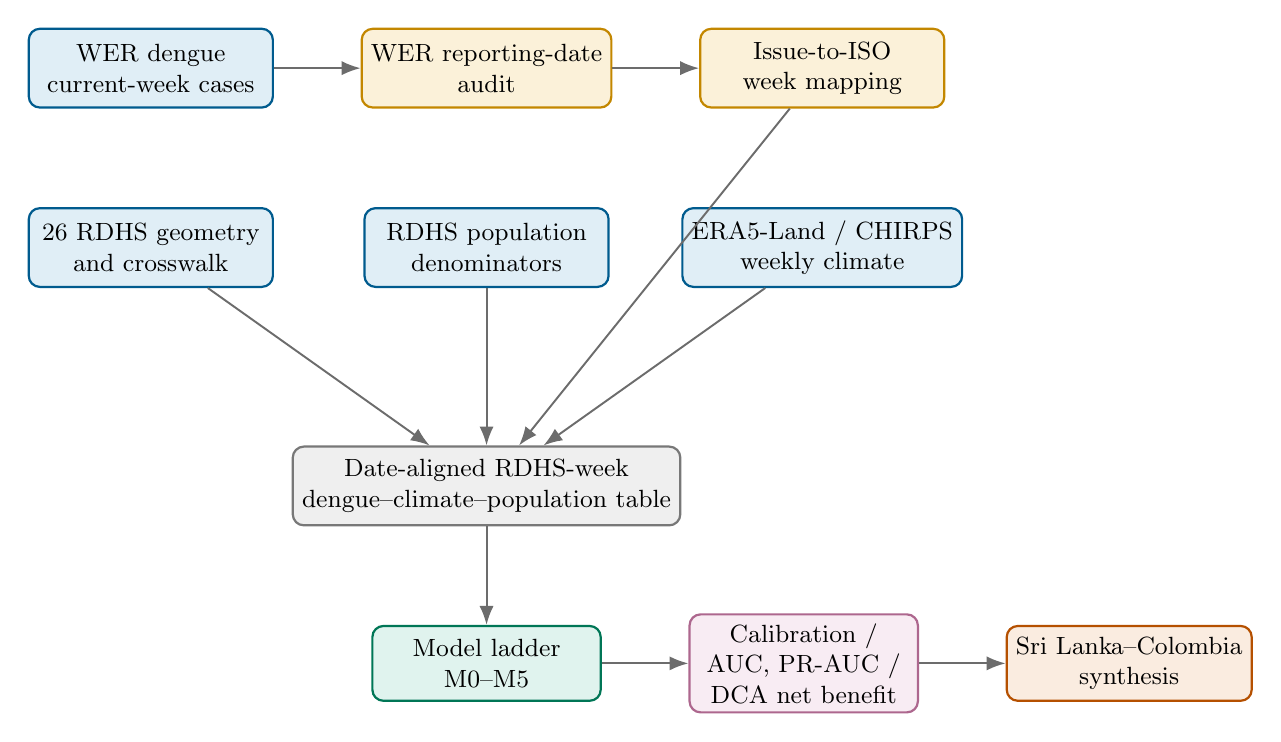
\begin{tikzpicture}[
    node distance=1.25cm and 1.1cm,
    every node/.style={font=\small},
    src/.style   ={rectangle, rounded corners, draw=okBlue!80!black, fill=okBlue!12, line width=0.8pt, align=center, minimum width=3.1cm, minimum height=1.0cm},
    pre/.style   ={rectangle, rounded corners, draw=okOrange!85!black, fill=okOrange!15, line width=0.8pt, align=center, minimum width=3.1cm, minimum height=1.0cm},
    integ/.style ={rectangle, rounded corners, draw=okGray, fill=okGray!12, line width=0.8pt, align=center, minimum width=4.6cm, minimum height=1.0cm},
    mod/.style   ={rectangle, rounded corners, draw=okGreen!75!black, fill=okGreen!12, line width=0.8pt, align=center, minimum width=2.9cm, minimum height=0.95cm},
    evaln/.style ={rectangle, rounded corners, draw=okPurple!85!black, fill=okPurple!14, line width=0.8pt, align=center, minimum width=2.9cm, minimum height=0.95cm},
    outnode/.style={rectangle, rounded corners, draw=okVermillion!85!black, fill=okVermillion!12, line width=0.8pt, align=center, minimum width=2.9cm, minimum height=0.95cm},
    arrow/.style ={-{Latex[length=2.4mm]}, line width=0.7pt, draw=okGray!90!black}
]
\node[src] (wer) {WER dengue\\current-week cases};
\node[pre, right=of wer] (date) {WER reporting-date\\audit};
\node[pre, right=of date] (iso) {Issue-to-ISO\\week mapping};
\node[src, below=of iso] (climate) {ERA5-Land / CHIRPS\\weekly climate};
\node[src, below=of date] (pop) {RDHS population\\denominators};
\node[src, below=of wer] (geom) {26 RDHS geometry\\and crosswalk};
\node[integ, below=2.0cm of pop] (linked) {Date-aligned RDHS-week\\dengue--climate--population table};
\node[mod, below=of linked] (models) {Model ladder\\M0--M5};
\node[evaln, right=of models] (eval) {Calibration /\\AUC, PR-AUC /\\DCA net benefit};
\node[outnode, right=of eval] (synth) {Sri Lanka--Colombia\\synthesis};
\draw[arrow] (wer) -- (date);
\draw[arrow] (date) -- (iso);
\draw[arrow] (iso) -- (linked);
\draw[arrow] (climate) -- (linked);
\draw[arrow] (pop) -- (linked);
\draw[arrow] (geom) -- (linked);
\draw[arrow] (linked) -- (models);
\draw[arrow] (models) -- (eval);
\draw[arrow] (eval) -- (synth);
\end{tikzpicture}
\caption{Study pipeline and WER-to-ISO week alignment. Reporting dates were used to map WER issues to ISO epidemiological weeks before joining dengue, climate, population, and spatial data.}
\label{fig:pipeline}
\end{figure}

\subsection{Sri Lanka primary comparison}
Among the initial M0--M3 benchmark comparison, in the held-out 2023--2025 test period the recent-case surveillance model M1 had the highest discrimination, lowest Brier score, and highest net benefit at $p^*=0.30$ (Table~\ref{tab:slprimary}). The climate-only and structured-climate models showed predictive signal but did not exceed M1. At $p^*=0.30$, M1 net benefit was 0.137, versus 0.069 (M2) and 0.078 (M3); alert-all was lower than M1 and alert-none was zero. Decision value was threshold-dependent (Table~\ref{tab:slthresh}, Fig~\ref{fig:sldca}): at low thresholds alert-all was competitive, as expected when the threshold lies well below test prevalence, while across the mid-to-high range M1 was consistently highest among M0--M3.

\begin{table}[htbp]
\centering
\caption{Initial Sri Lanka M0--M3 benchmark comparison ($h=4$, RDHS 75th-percentile alert label, 2023--2025 test period). Hybrid models M4--M5 are reported separately.}
\label{tab:slprimary}
\begin{threeparttable}\footnotesize
\setlength{\tabcolsep}{3.6pt}
\begin{tabular}{llrrrrrrrr}
\toprule
Model & Description & AUC & PR-AUC & Brier & CITL & Slope & Mean pred. & Obs. & NB$_{0.30}$ \\
\midrule
M0 & Seasonal climatology & 0.629 & 0.459 & 0.222 & +0.530 & 0.664 & 0.238 & 0.336 & 0.084 \\
M1 & Recent-case surveillance & 0.752 & 0.652 & 0.191 & +0.513 & 1.246 & 0.246 & 0.336 & 0.137 \\
M2 & Climate-only & 0.643 & 0.460 & 0.220 & +0.479 & 1.027 & 0.243 & 0.336 & 0.069 \\
M3 & Climate + season + RDHS FE & 0.652 & 0.476 & 0.220 & +0.596 & 0.738 & 0.229 & 0.336 & 0.078 \\
\bottomrule
\end{tabular}
\begin{tablenotes}\footnotesize
\item AUC, area under the receiver-operating characteristic curve; PR-AUC, area under the precision--recall curve; Brier, Brier score; CITL, calibration-in-the-large; Slope, calibration slope; Mean pred., mean predicted probability; Obs., observed prevalence; NB$_{0.30}$, net benefit at the primary reference threshold $p^*=0.30$; FE, fixed effects.
\end{tablenotes}
\end{threeparttable}
\end{table}

\begin{table}[htbp]
\centering
\caption{Sri Lanka net benefit at representative decision thresholds.}
\label{tab:slthresh}
\small
\begin{tabular}{rrrrrrr}
\toprule
Threshold $p^*$ & Alert-all & Alert-none & M0 & M1 & M2 & M3 \\
\midrule
0.20 & 0.171 & 0.000 & 0.161 & 0.185 & 0.164 & 0.147 \\
0.30 & 0.052 & 0.000 & 0.084 & 0.137 & 0.069 & 0.078 \\
0.34 & $-0.005$ & 0.000 & 0.059 & 0.111 & 0.032 & 0.060 \\
0.40 & $-0.106$ & 0.000 & 0.025 & 0.083 & 0.012 & 0.039 \\
\bottomrule
\end{tabular}
\end{table}

\begin{figure}[htbp]
\centering
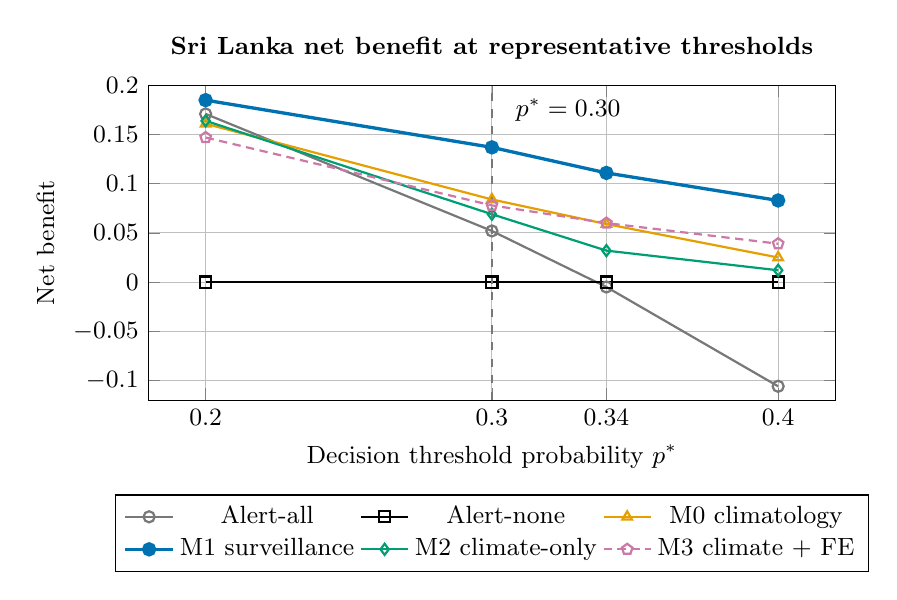
\begin{tikzpicture}
\begin{axis}[
    width=0.85\textwidth, height=0.46\textwidth,
    xlabel={Decision threshold probability $p^*$}, ylabel={Net benefit},
    xmin=0.18, xmax=0.42, ymin=-0.12, ymax=0.20,
    xtick={0.20,0.30,0.34,0.40}, ytick={-0.10,-0.05,0,0.05,0.10,0.15,0.20},
    grid=both, tick label style={font=\small}, label style={font=\small},
    legend style={at={(0.5,-0.30)}, anchor=north, legend columns=3, font=\small},
    title={Sri Lanka net benefit at representative thresholds}, title style={font=\small\bfseries}]
\addplot+[mark=o, thick, color=okGray] coordinates {(0.20,0.171)(0.30,0.052)(0.34,-0.005)(0.40,-0.106)}; \addlegendentry{Alert-all}
\addplot+[mark=square, thick, color=black] coordinates {(0.20,0)(0.30,0)(0.34,0)(0.40,0)}; \addlegendentry{Alert-none}
\addplot+[mark=triangle, thick, color=okOrange] coordinates {(0.20,0.161)(0.30,0.084)(0.34,0.059)(0.40,0.025)}; \addlegendentry{M0 climatology}
\addplot+[mark=*, very thick, color=okBlue] coordinates {(0.20,0.185)(0.30,0.137)(0.34,0.111)(0.40,0.083)}; \addlegendentry{M1 surveillance}
\addplot+[mark=diamond, thick, color=okGreen] coordinates {(0.20,0.164)(0.30,0.069)(0.34,0.032)(0.40,0.012)}; \addlegendentry{M2 climate-only}
\addplot+[mark=pentagon, thick, color=okPurple] coordinates {(0.20,0.147)(0.30,0.078)(0.34,0.060)(0.40,0.039)}; \addlegendentry{M3 climate + FE}
\addplot[dashed, thick, color=okGray] coordinates {(0.30,-0.12)(0.30,0.20)};
\node[anchor=west, font=\small] at (axis cs:0.305,0.175) {$p^*=0.30$};
\end{axis}
\end{tikzpicture}
\caption{Sri Lanka net benefit at representative decision thresholds ($h=4$, 75th-percentile label). Points are net benefit at four representative thresholds (Table~\ref{tab:slthresh}); line segments connect them and do not represent a recomputed continuous grid. The 0.34 threshold brackets the alert-all zero-crossing (alert-all net benefit $-0.005$ there, near the test prevalence of 0.336) and is included as a representative diagnostic threshold, not a selected operating point. The recent-case surveillance model (M1) had the highest net benefit at $p^*=0.30$ and across the evaluated mid-to-high threshold range. Colorblind-safe (Okabe--Ito) palette.}
\label{fig:sldca}
\end{figure}

\subsection{Calibration and recalibration}
All M0--M3 models in the initial comparison under-predicted in the test period (CITL $+0.530$ M0, $+0.513$ M1, $+0.479$ M2, $+0.596$ M3; mean predicted $\approx$0.23--0.25 against observed prevalence 0.336), consistent with the 24.2\%$\rightarrow$33.6\% training-to-test prevalence shift. The hybrid models M4 and M5 also under-predicted in the test period (CITL $+0.449$ and $+0.440$, calibration slopes 1.225 and 1.077), so the under-prediction was not confined to the initial benchmark ladder. Rolling 52-week intercept-only recalibration substantially reduced calibration-in-the-large error for all four M0--M3 benchmark-ladder models (restricted to the M0--M3 ladder; the primary hybrid models M4 and M5 were therefore \emph{not} recalibrated, so the Sri Lanka $\Delta$NB(M4$-$M1) and $\Delta$NB(M5$-$M1) are internally consistent raw-vs-raw comparisons rather than the calibrated contrast the evaluation otherwise advocates---a limitation), leaving residual CITL of $+0.029$ (M0), $+0.020$ (M1), $+0.046$ (M2), and $+0.087$ (M3) (Table~\ref{tab:recal}), and outperformed expanding-window recalibration, which under-corrected. Intercept-only recalibration addresses average under- or over-prediction but does not by itself correct calibration slope or nonlinear miscalibration, so it does not imply perfect calibration; for example, M3's residual CITL was $+0.087$. No recalibration fallbacks occurred. Recalibration did not change the model ranking: across the evaluated recalibration methods M1 net benefit at $p^*=0.30$ ranged 0.124--0.142 while the maximum recalibrated climate-only (M2/M3) net benefit was approximately 0.085, so reducing calibration error did not make climate-only models exceed surveillance.

\begin{table}[htbp]
\centering
\caption{Calibration-in-the-large before and after time-updated recalibration.}
\label{tab:recal}
\small
\begin{tabular}{lrrrr}
\toprule
Model & Raw CITL & Rolling-52 & Rolling-104 & Expanding \\
\midrule
M0 & +0.530 & +0.029 & +0.137 & +0.338 \\
M1 & +0.513 & +0.020 & +0.111 & +0.325 \\
M2 & +0.479 & +0.046 & +0.155 & +0.314 \\
M3 & +0.596 & +0.087 & +0.204 & +0.394 \\
\bottomrule
\end{tabular}
\end{table}

\subsection{Sri Lanka structured-climate and hybrid results}
The Python DLNM-style and canonical R \texttt{dlnm} climate specifications produced nearly identical performance: the Python DLNM-style minus canonical R-DLNM differences in AUC and in net benefit at $p^*=0.30$ were near zero. Both climate specifications remained below the recent-surveillance benchmark M1. For the canonical R DLNM minus M1, the signed contrasts were $\Delta$AUC(R\nobreakdash-DLNM$-$M1) $=-0.038$ (95\% CI $-0.066$ to $-0.008$) and $\Delta$NB(R\nobreakdash-DLNM$-$M1) at $p^*=0.30$ $=-0.025$ (95\% CI $-0.041$ to $-0.006$); that is, the canonical R-DLNM climate model was lower than M1 on both (M1 net benefit 0.137 versus 0.112 for the canonical R DLNM) (Table~\ref{tab:dlnmhybrid}). For the planned primary hybrid (M4), the M4$-$M1 net-benefit estimate at $p^*=0.30$ was $-0.008$ (95\% CI $-0.028$ to $+0.013$; the rounded per-model table entries differ by $-0.009$, and $-0.008$ is the bootstrap point estimate) and $\Delta$AUC(M4$-$M1) was $+0.013$ (95\% CI $-0.020$ to $+0.046$). The expanded sensitivity hybrid M5 (adding seasonal harmonics and geographic fixed effects to M4) reached AUC 0.772, PR-AUC 0.667, Brier 0.180 (CITL $+0.440$, calibration slope 1.077; M4 CITL $+0.449$, slope 1.225), and net benefit 0.145 at $p^*=0.30$ (M1: 0.752, 0.652, 0.191, 0.137); the M5$-$M1 net-benefit estimate at $p^*=0.30$ was $+0.0081$ (95\% CI $-0.0012$ to $+0.0181$), a small positive point estimate with substantial uncertainty (Table~\ref{tab:dlnmhybrid}; see the cross-setting summary). As with the Colombia expanded hybrid, the Sri Lanka M5 added seasonal harmonics and RDHS-level fixed effects that M1 does not contain, so the Sri Lanka M5$-$M1 contrast should also be interpreted as a compound augmentation rather than a climate-specific increment; no analogous specification-matched decomposition was conducted for Sri Lanka. A secondary wild-cluster-bootstrap-t analysis using all 26 RDHS clusters produced uncertainty intervals similar to the original percentile cluster-bootstrap intervals for both the planned M4$-$M1 and expanded M5$-$M1 contrasts (Supporting Information, S11 Table and S12 Text).

\begin{table}[htbp]
\centering
\caption{Sri Lanka climate-only, distributed-lag, and hybrid model comparison (test period, $h=4$, 75th-percentile label). Net benefit is shown at representative thresholds. M4 is the planned primary hybrid; M5 is the expanded sensitivity hybrid (adding seasonal harmonics and geographic fixed effects to M4).}
\label{tab:dlnmhybrid}
\small
\begin{tabular}{lrrrr}
\toprule
Model & AUC & NB$_{0.20}$ & NB$_{0.30}$ & NB$_{0.40}$ \\
\midrule
M1 recent-case surveillance & 0.752 & 0.185 & 0.137 & 0.083 \\
M2 climate-only & 0.643 & 0.164 & 0.069 & 0.012 \\
M3 climate + season/RDHS & 0.652 & 0.147 & 0.078 & 0.039 \\
Python DLNM-style climate & 0.714 & 0.179 & 0.111 & 0.057 \\
Canonical R DLNM climate & 0.714 & 0.181 & 0.112 & 0.053 \\
M4 planned primary hybrid & 0.764 & 0.193 & 0.128 & 0.087 \\
M5 expanded sensitivity hybrid & 0.772 & 0.194 & 0.145 & 0.107 \\
\bottomrule
\end{tabular}
\end{table}

\subsection{Colombia: a second, differently-constructed case study}
The Colombia primary $h=4$ analysis used a common-complete test set (n${}=13{,}361$; test prevalence 0.375) on which models M0--M5 were all evaluated, with the complete-case intersection defined by the M1--M5 predictors; the split was training 2006--2017, validation 2018--2019, and test 2020--2022. As in Sri Lanka, climate-only models were weak (M2 AUC 0.556, M3 0.564) relative to M1 (AUC 0.685). The hybrid had a higher net-benefit point estimate than M1: M5 AUC 0.726 and net benefit 0.136 at $p^*=0.30$ versus M1 0.685 and 0.117, with municipality-cluster bootstrap $\Delta$AUC $+0.040$ (95\% CI $+0.024$ to $+0.058$) and $\Delta$NB at $p^*=0.30$ $+0.0188$ (95\% CI $+0.0117$ to $+0.0260$) (Table~\ref{tab:colombia}, Fig~\ref{fig:colombia}). This full-hybrid M5$-$M1 contrast combined climate with seasonal terms and 32 department fixed effects that M1 does not contain, and therefore did not isolate the climate contribution; a post hoc specification-matched decomposition of this compound difference is reported below (see ``Specification-matched decomposition of the full hybrid contrast''). At $p^*=0.30$, the compound $\Delta$NB of $+0.0188$ corresponds to approximately 1.9 additional net true-positive equivalents per 100 municipality-weeks (approximate interval 1.2 to 2.6 per 100). Equivalently---rather than additionally---holding true-positive detections fixed, it corresponds to approximately 4.4 fewer false-alert equivalents per 100 municipality-weeks (approximate interval 2.7 to 6.1 per 100). Both intervals are monotone rescalings of the same pointwise, multiplicity-unadjusted $\Delta$NB confidence interval and inherit its caveats. These are alternative decision-analytic representations of the same net-benefit difference, not observed numbers of outbreaks detected, alerts prevented, cases prevented, or lives saved. The Colombia test period (2020--2022) includes the COVID-19-era years 2020--2021. Platt recalibration was fit on the validation period, and the calibration metrics reported here are after that recalibration. All models nonetheless over-predicted in the test period: calibration-in-the-large remained negative for every model (M0 $-0.50$, M1 $-0.46$, M2 $-0.50$, M3 $-0.54$, M4 $-0.45$, M5 $-0.50$), with Brier scores 0.213--0.250, consistent with the temporal prevalence shift not being fully removed by validation-fit recalibration. Colombia calibration slopes ranged from 0.85 to 3.43 across the model ladder; the extremes were the climatology baseline M0 (slope 3.43) and the climate-only baseline M2 (slope 0.85), whereas the models carrying the net-benefit comparison---M1, M4, and M5---had slopes near 1 (1.09, 1.05, and 1.16). M0, M2 and M3 had net benefit approximately equal to the alert-all strategy and below M1, M4 and M5. Although M1 and M5 were evaluated on the same test observations and under the same validation-fit recalibration framework, both retained test-period calibration error. Their net-benefit contrast should therefore be interpreted together with the reported calibration-in-the-large, calibration-slope and Brier-score results. Observed prevalence was 0.375 for the common-complete test set, which was shared by all models; per-model mean predicted probability was not retained in the committed reproducibility record. The within-test M5-versus-M1 contrast is reported with this calibration limitation.

\subsubsection*{Specification-matched decomposition of the full hybrid contrast}
To separate the climate contribution from the non-climate structure inside the compound M5$-$M1 difference, we conducted a post hoc specification-matched decomposition in the original Colombia pipeline, using the identical row set, model family, tuning, validation-fit recalibration, and municipality-cluster bootstrap. We defined a matched baseline, M5$_{\text{no-climate}}$, containing recent-case terms, seasonal terms, and the 32 department fixed effects---identical to M5 except that the 18 climate columns were removed. All models were evaluated on the identical common-complete test set ($n=13{,}361$) at $p^*=0.30$ (Table~\ref{tab:matcheddecomp}).

Adding climate to the matched baseline contributed $\Delta$NB(M5$-$M5$_{\text{no-climate}}$) $=+0.0078$ (95\% CI $+0.0039$ to $+0.0119$): a small increment that remained distinguishable from zero under conditional test-set resampling (its 95\% interval excludes zero; this conditional interval omits model-development uncertainty and is therefore optimistically narrow) but was roughly half the compound $+0.0188$. Adding seasonal terms and department fixed effects to M1 contributed $\Delta$NB(M5$_{\text{no-climate}}-$M1) $=+0.0110$ (95\% CI $+0.0060$ to $+0.0164$). Separately, adding climate to a cases-only baseline gave $\Delta$NB(M4$-$M1) $=+0.0122$ (95\% CI $+0.0073$ to $+0.0171$); this cases-only climate contrast does not control for seasonal and department-level structure and therefore does not estimate an independent climate effect. In a structure-first sequence, adding seasonality and department fixed effects to M1 increased net benefit by $+0.0110$, after which adding climate increased it by a further $+0.0078$; these sequential shares are path-dependent and are not unique causal allocations. In a paired municipality-cluster bootstrap, climate's marginal net-benefit contribution was larger when added to a cases-only baseline than when added to the structure-matched baseline (difference $+0.0044$, 95\% CI $+0.0008$ to $+0.0081$), indicating that part of the apparent climate value overlapped with seasonal and geographic structure. Because a single sequential ordering is arbitrary, we summarize the attribution with an order-averaged (Shapley) value over the two orderings, which assigned climate approximately $+0.0100$ (95\% CI $+0.0060$ to $+0.0142$) and non-climate structure approximately $+0.0087$ of the $+0.0188$ compound difference; we therefore do not report a fixed percentage split. Because $p^*=0.30$ was not elicited from stakeholders or derived from documented response costs, we summarize net benefit across the evaluated decision-curve grid rather than relying on a single threshold~\cite{VanCalster2019,Vickers2016}. Across the grid ($p^*=0.05$--$0.50$), the compound $\Delta$NB(M5$-$M1) averaged $+0.0118$ and rose with the threshold (near zero for $p^*\le0.15$, $+0.0188$ at $0.30$, and $+0.0251$ at $0.40$), a pattern consistent with threshold and prevalence sensitivity rather than a threshold-invariant climate effect; the qualitative conclusions were unchanged across the evaluated range. This decomposition was a post hoc specification-matching diagnostic; the robustness of the residual increment is examined next. Full feature lists, the removed climate columns, the retained terms, row identity, and the bootstrap protocol are provided in Supporting Information.

\subsubsection*{Robustness of the Colombia climate increment}
We examined whether the residual \emph{matched} climate increment, $\Delta$NB(M5$-$M5$_{\text{no-climate}}$), is stable, re-computing that same matched contrast in each test (the primary compound $+0.0188$ and matched increment ($+0.0079$ as a full-precision bootstrap point estimate; $+0.0078$ as the rounded Table~6 difference) were reproduced to $<0.0001$ by the reimplementation beforehand). The evidence is mixed and does not, on its own, establish robustness. (i) \emph{Functional form.} Refitting the climate terms as a distributed-lag nonlinear cross-basis (natural-spline value $\times$ lag bases) in temperature and precipitation left the increment somewhat \emph{larger}, not smaller ($+0.0122$, 95\% CI $+0.0078$ to $+0.0160$; coincidentally equal to the cases-only M4$-$M1 point estimate, though the two are distinct contrasts with different intervals); the increment is therefore not an artifact of the linear-lag form, though this is the least-threatening robustness dimension. Humidity was unavailable for Colombia and could not be added, so this test varies the functional form, not the variable set. (ii) \emph{Reporting delay.} Emulating reporting delay by censoring the most recent case lags---degrading the surveillance predictors while holding the outcome label and climate vintages at their finalized values---the matched increment \emph{decayed monotonically}: $+0.0079$ uncensored, $+0.0077$ (95\% CI $+0.0034$ to $+0.0132$) at a two-week lag, and $+0.0049$ (95\% CI $+0.0001$ to $+0.0097$) at a three-week lag, its lower confidence bound falling to essentially zero. Because operational dengue reporting is delayed by weeks and even ``final'' climate products lag (CHIRPS $\approx$3 weeks, ERA5-Land 2--3 months), the operating regime with delayed surveillance is where the climate-specific increment approaches zero; we read this as a limitation, not as support. (The \emph{compound} $\Delta$NB(M5$-$M1) instead grew under censoring, but that reflects degradation of the recent-case baseline, not a climate-specific gain.) (iii) \emph{Pre-pandemic period.} On a single pre-specified pre-pandemic split (train $\le$2015, validation 2016--2017, test 2018--2019, test data excluded from training and recalibration), the matched increment was $+0.0199$ (95\% CI $+0.0012$ to $+0.0400$)---the same sign but larger and barely excluding zero. This window is not endemic-baseline evidence: recalibration is fit on 2016, the dengue--Zika co-circulation year in which clinical misclassification distorted dengue surveillance, and evaluated on 2019, Colombia's largest recent epidemic, at high prevalence ($\approx0.50$) where alert-all is competitive; the inflated value is possibly an epidemic-amplitude confound (one of several directions in which a high-prevalence, Zika-co-circulating year could bias the estimate). (iv) \emph{No clean post-pandemic test.} The pandemic-window question could be probed by re-evaluating the matched contrast on \emph{post-pandemic} 2023 data (within the cited OpenDengue v1.3 but beyond the 2020--2022 archive analysed here, requiring re-acquisition). This was not done, and it would not be a clean test: 2023 was a record dengue-epidemic year in the Americas (over 4.2 million cases, surpassing the 2019 record), with Colombia among the hardest hit~\cite{PAHO2023}; contemporaneous reports document DENV-3 lineage introductions in Colombia~\cite{ValleDelCauca2024} under climatic conditions coinciding with the 2023--2024 El Ni\~no, so a 2023 evaluation would carry its own epidemic-amplitude confound (mirroring the 2019 problem) and, because OpenDengue counts are finalized, could not address the reporting-delay dimension under which the increment attenuated toward zero. It therefore remains a partial, itself-confounded check rather than a definitive tiebreaker. Taken together---one uninformative pass (functional form), one dimension where it attenuated toward zero (a surveillance-lag feature-censoring sensitivity, three-week matched $+0.0049$, 95\% CI $+0.0001$ to $+0.0097$), one uninterpretable pass (a Zika- and epidemic-confounded pre-pandemic window), and one missing test (post-pandemic)---the evidence does not support a robust climate increment. The single conclusion the data support is that, \emph{in the two settings tested, no climate increment survived realistic conditions}: Sri Lanka was null, and the Colombia increment appeared only under finalized counts, an unmatched baseline, and a pandemic-era window. We therefore subordinate the residual $+0.0078$ and make no claim of a robust or transportable climate benefit. These sensitivity analyses used a Python reimplementation of the frozen pipeline (reproducing the primary estimate exactly); reporting delay was emulated by feature censoring, not true reporting triangles. Because the emulation degraded only the surveillance predictors while holding climate at finalized, best-case vintages (final CHIRPS lags $\approx$3 weeks and ERA5-Land 2--3 months, though preliminary products exist at days' latency), the attenuation toward zero under delay is conservative: the matched climate increment's estimated decision value approached zero even when climate was held at its most favorable vintages. The point concerns decision value, not climate-data availability.

\begin{table}[H]
\centering
\caption{Colombia specification-matched decomposition (post hoc diagnostic), $h=4$, 75th-percentile label, common-complete test set ($n=13{,}361$, prevalence 0.375), at $p^*=0.30$. Net benefit (NB) on validation-recalibrated predictions. The matched baseline (M5$_{\text{no-climate}}$) differs from M5 only by the 18 climate columns. Contrasts (in text) use municipality-cluster percentile bootstrap 95\% CIs (seed 20260612, $B=1000$, zero failures). This is an additional post hoc analysis, not a prespecified or confirmatory one.}
\label{tab:matcheddecomp}
\begin{tabular}{llrr}
\toprule
Model & Information set & Features & NB@$0.30$ \\
\midrule
M1 & cases & 4 & 0.1171 \\
M5$_{\text{no-climate}}$ (matched) & cases $+$ season $+$ dept.\ FE & 40 & 0.1280 \\
M4 & cases $+$ climate & 22 & 0.1293 \\
M5 & cases $+$ climate $+$ season $+$ dept.\ FE & 58 & 0.1358 \\
\bottomrule
\end{tabular}
\end{table}

\begin{table}[htbp]
\centering
\caption{Colombia $h=4$ primary common-complete test performance (second, differently-constructed case study). Net benefit at $p^*=0.30$; alert-all reference $\approx$0.107, alert-none $0$. Test prevalence was 0.375 for the common-complete set shared by M0--M5. Per-model values for all six ladder models (M0--M5) are shown for completeness. The compound M5$-$M1 contrast combines climate with seasonal and department fixed-effect structure and is not a climate-specific effect; the climate-specific increment and the M4$-$M1 contrast are reported in the specification-matched decomposition below (Table~\ref{tab:matcheddecomp}). Per-model mean predicted probabilities were not retained in the committed reproducibility record. Calibration-in-the-large, calibration slope, and Brier-score results are summarized in the text and Supporting Information.}
\label{tab:colombia}
\small
\begin{tabular}{llrr}
\toprule
Model & Description & AUC & NB$_{0.30}$ \\
\midrule
M0 & Seasonal climatology & 0.513 & 0.108 \\
M1 & Recent-case surveillance & 0.685 & 0.117 \\
M2 & Climate-only & 0.556 & 0.108 \\
M3 & Climate + seasonality + department fixed effects & 0.564 & 0.108 \\
M4 & Recent cases + linear climate lags (no seasonality or fixed effects) & 0.699 & 0.129 \\
M5 & Hybrid climate + surveillance & 0.726 & 0.136 \\
\midrule
\multicolumn{2}{l}{Alert-all reference} & --- & $\approx$0.107 \\
\bottomrule
\end{tabular}
\end{table}

\noindent In the primary common-complete analysis, M2 and M3 had net benefit close to alert-all ($\approx$0.107) and below M1. In a separate, larger climate-only row set their net benefit was approximately 0.001 (AUC $\approx$0.532 and 0.546), indicating that climate-only weakness was not an artifact of the common-complete subset. Because the analyses used different denominators, they are reported separately.

\begin{figure}[htbp]
\centering
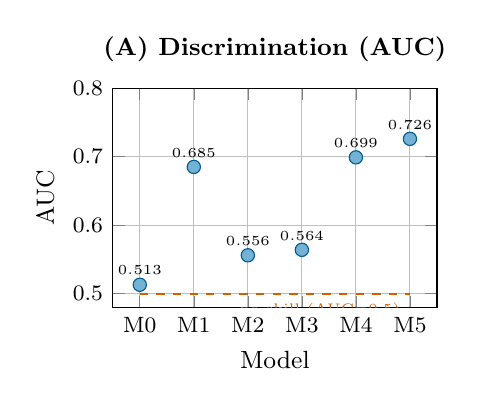
\begin{tikzpicture}
\begin{axis}[
    width=0.47\textwidth, height=0.36\textwidth,
    symbolic x coords={M0,M1,M2,M3,M4,M5}, xtick=data, ymin=0.48, ymax=0.80, ytick={0.5,0.6,0.7,0.8},
    ylabel={AUC}, xlabel={Model}, grid=both,
    tick label style={font=\footnotesize}, label style={font=\small},
    title={(A) Discrimination (AUC)}, title style={font=\small\bfseries},
    nodes near coords, every node near coord/.append style={font=\tiny, anchor=south},
    nodes near coords style={/pgf/number format/.cd, fixed, precision=3}]
\draw[dashed, thick, draw=okVermillion] ({axis cs:M0,0.5}) -- ({axis cs:M5,0.5});
\node[anchor=north east, font=\tiny, text=okVermillion] at (axis cs:M5,0.5) {no-skill (AUC$=$0.5)};
\addplot[only marks, mark=*, mark size=2.4pt, draw=okBlue!80!black, fill=okBlue!55] coordinates {(M0,0.513)(M1,0.685)(M2,0.556)(M3,0.564)(M4,0.699)(M5,0.726)};
\end{axis}
\end{tikzpicture}\hfill
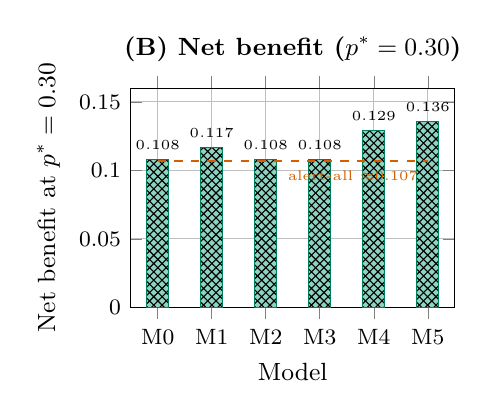
\begin{tikzpicture}
\begin{axis}[
    width=0.47\textwidth, height=0.36\textwidth, ybar, bar width=8pt,
    symbolic x coords={M0,M1,M2,M3,M4,M5}, xtick=data, ymin=0, ymax=0.16, ytick={0,0.05,0.10,0.15},
    ylabel={Net benefit at $p^*=0.30$}, xlabel={Model}, grid=both,
    tick label style={font=\footnotesize}, label style={font=\small},
    title={(B) Net benefit ($p^*=0.30$)}, title style={font=\small\bfseries},
    nodes near coords, every node near coord/.append style={font=\tiny},
    nodes near coords style={/pgf/number format/.cd, fixed, precision=3}]
\addplot[fill=okGreen!45, draw=okGreen!80!black, postaction={pattern=crosshatch}] coordinates {(M0,0.108)(M1,0.117)(M2,0.108)(M3,0.108)(M4,0.129)(M5,0.136)};
\draw[dashed, thick, draw=okVermillion] ({axis cs:M0,0.107}) -- ({axis cs:M5,0.107});
\node[anchor=north east, font=\tiny, text=okVermillion] at (axis cs:M5,0.107) {alert-all $\approx$0.107};
\end{axis}
\end{tikzpicture}
\caption{Colombia model-ladder discrimination and net benefit ($h=4$, common-complete test set, $n=13{,}361$). (A) AUC and (B) net benefit at $p^*=0.30$ for models M0--M5. Panel~A is a dot plot with a dashed reference line at the no-skill value (AUC${}=0.5$), the meaningful baseline for discrimination, with exact three-decimal AUC values labeled above each point (no truncated bars). Panel B uses a zero-based axis so that the alert-none reference (net benefit $=0$) is the baseline and the alert-all reference ($\approx$0.107, dashed line) and the small between-model differences are shown in true proportion; exact three-decimal values are labeled above each bar. Climate-only models (M2, M3) had net benefit close to alert-all and below M1; M5 had the highest AUC and net benefit. Values are transcribed from Table~\ref{tab:colombia}; Panel~B bars use a redundant hatch pattern and Panel~A uses filled circular markers for grayscale legibility.}
\label{fig:colombia}
\end{figure}

\subsection{Horizon result}
Across the tested Colombia horizons, the M5$-$M1 net-benefit increment was approximately flat rather than increasing with lead time: $\Delta$NB(M5$-$M1) was approximately $+0.015$ to $+0.019$ across $h=1$--8 and approximately $+0.014$ at $h=12$, while $\Delta$AUC fell from approximately $+0.040$ ($h\le4$) to approximately $+0.024$ ($h=12$). In Sri Lanka, no model reliably exceeded the recent-surveillance baseline (M1) in net benefit at $p^*=0.30$ across the evaluated label--horizon cells (the expanded hybrid M5 point estimate was marginally higher at the primary cell, with an interval spanning zero); M1 discrimination declined with horizon (AUC 0.843, 0.810, 0.752, 0.679, 0.646 at $h=1,2,4,8,12$ for the 75th-percentile label), with climate models narrowing the discrimination gap at long horizons as M1's own discrimination decayed, without overturning the net-benefit result. The Sri Lanka and Colombia horizon analyses estimate related but not identical quantities. Together, these findings provided no evidence that climate delivered increasing decision value over the tested 1--12-week range. These results are scoped to short-to-medium lead times; climate information has shown forecasting skill for dengue at longer, seasonal (3--6-month) horizons, where autoregressive signal decays~\cite{Beal2025,ColonGonzalez2021}---indeed \cite{Beal2025} report hydroclimate skill at 3--6-month leads in Colombian cities, directly complementary to our null at 1--12-week leads in Colombia, so our null is scope-limited to short-to-medium lead--- and operational seasonal systems (for example the D-MOSS system in Vietnam~\cite{Campbell2026}) target longer, 4--6-month lead times, where D-MOSS reports its greatest value-added over seasonal-average baselines, so our conclusions should be read as pertaining to short-to-medium-lead elevated-activity alerting rather than as evidence against climate value at seasonal scales.

\subsection{Threshold and stricter-outcome robustness}
In Sri Lanka, a secondary targeted-value analysis across train-defined regimes found the all-test $\Delta$NB(M5$-$M1) at $p^*=0.30$ was $+0.0081$ (95\% CI $-0.0012$ to $+0.0181$); the regime estimates were small with wide, pointwise, multiplicity-unadjusted intervals, and the largest regime estimate (high-incidence $\times$ strong-autocorrelation, $+0.0202$) was interpreted as exploratory; because it was based on only eight clusters, the associated percentile interval is not interpretable as a valid bootstrap confidence interval and the estimate is reported as a point value only. At $p^*=0.40$, the all-test $\Delta$NB(M5$-$M1) estimate was $+0.0241$ (95\% CI $+0.0090$ to $+0.0399$), compared with $+0.0081$ at the primary reference threshold of $p^*=0.30$ and $+0.0096$ (95\% CI $-0.0005$ to $+0.0187$) at $p^*=0.20$. This was a secondary threshold-specific analysis; the evaluated-grid estimates were pointwise and unadjusted for multiplicity. Incremental net benefit was larger at the higher evaluated threshold ($p^*=0.40$) than at $p^*=0.30$ or $p^*=0.20$, although these secondary estimates are interpreted descriptively rather than as separate hypothesis tests; the evaluated $p^*=0.20/0.30/0.40$ estimates are those reported in this paragraph. In Colombia, the secondary stricter exceedance-threshold sensitivity (training-referenced 75th/80th/90th-percentile labels) gave $\Delta$NB(M5$-$M1) at $p^*=0.30$ of $+0.0188$ (95\% CI $+0.0117$ to $+0.0260$), $+0.0157$ (95\% CI $+0.0082$ to $+0.0236$), and $+0.0092$ (95\% CI $+0.0003$ to $+0.0183$); the estimates attenuated from $+0.0188$ at the 75th-percentile definition to $+0.0092$ at the 90th-percentile definition, and all intervals are pointwise and unadjusted for multiplicity. Even at the 90th-percentile definition the test-period prevalence of elevated-activity weeks remained approximately 23.5\%, so these are not evidence for rare-epidemic prediction. The 75th-percentile $h=4$ contrast remains the primary analysis; its operational translation is reported in the primary Colombia Results above.

In a secondary evaluation restricted to 2022, excluding observations from 2020--2021, the M5$-$M1 net-benefit estimate at $p^*=0.30$ was $+0.0150$ (95\% percentile interval $+0.0067$ to $+0.0249$), compared with $+0.0188$ in the full 2020--2022 test period. The 2022 subset contained 4{,}802 municipality-weeks from 274 municipalities, with 2{,}202 elevated-activity events and prevalence 0.4586. Because prevalence was higher in 2022, alert-all was substantially more competitive (alert-all net benefit $\approx$0.227 in the 2022 subset, against $\approx$0.107 in the full test period), so absolute net-benefit levels in the subset are higher and are not directly comparable to the full-period levels; the within-subset M5$-$M1 contrast is the comparable quantity. This subset was not interpreted as pandemic-free or post-pandemic validation. The subset contained 48 eligible prediction-origin weeks, from January 2 to November 27, 2022, rather than 52: under the four-week-ahead horizon the four December-2022 origin weeks would require four-week-ahead outcomes dated in January 2023, beyond the available target period (the latest target used corresponds to the November 27, 2022 origin, that is, December 25, 2022). Full per-model metrics, the M4$-$M1 subset estimate, and the origin/target date evidence are in Supporting Information (S9 Table).

\subsection{Cross-setting synthesis}
The Sri Lanka and Colombia hybrid estimates are shown side by side in Table~\ref{tab:crosssetting}. In Sri Lanka, the M5$-$M1 net-benefit estimate was $+0.0081$, with a 95\% CI from $-0.0012$ to $+0.0181$. In Colombia, the M5$-$M1 estimate was $+0.0188$, with a 95\% CI from $+0.0117$ to $+0.0260$. No formal interaction or heterogeneity analysis was performed, and equivalence was not assessed. The setting-specific estimates differed in magnitude and precision, but this study does not establish whether the underlying effects differ between settings. The two settings should therefore be interpreted as complementary evaluations rather than as a formal comparative experiment. Recent surveillance was a strong benchmark in both settings; climate-only models added limited decision value in both; and the hybrid increment was modest and varied in magnitude and precision across the evaluated settings.

\begin{table}[htbp]
\centering
\caption{Descriptive cross-setting expanded-hybrid estimates, $\Delta$NB(M5$-$M1), at the reference $h=4$, 75th-percentile definition and $p^*=0.30$. M5 was the pre-computation expanded sensitivity hybrid in Sri Lanka. These estimates are presented descriptively and were not a jointly prespecified cross-country estimand. No interaction or heterogeneity test was performed. 95\% CIs are percentile bootstrap and pointwise. The estimates therefore should not be interpreted as establishing a between-setting difference. The settings differ in period, spatial units, sample size, and climate-feature implementation.}
\label{tab:crosssetting}
\small
\begin{tabular}{lrr}
\toprule
Setting & $\Delta$NB(M5$-$M1) & 95\% CI \\
\midrule
Sri Lanka (RDHS-cluster bootstrap, all-test) & +0.0081 & $-0.0012$ to $+0.0181$ \\
Colombia (municipality-cluster bootstrap) & +0.0188 & $+0.0117$ to $+0.0260$ \\
\bottomrule
\end{tabular}
\end{table}

\subsection{Additional sensitivity, selection, and validation analyses}

\subsubsection*{Recalibration sensitivity of the primary Sri Lanka contrast}
Because rolling recalibration was applied only to the M0--M3 ladder, we assessed whether recalibrating the hybrids changes the primary conclusion. Using an out-of-fold, cross-fitted (ISO-week-parity two-fold) Platt recalibration (leakage-controlled but internal and optimistic, since it uses concurrent test-period weeks rather than a past-only operational procedure) of the frozen Sri Lanka test predictions for M1, M4, and M5, calibration-in-the-large was corrected from CITL $+0.44$ to $+0.51$ (raw) to $\approx0$ and slopes to $\approx1$. The raw net-benefit gap then closed: $\Delta$NB(M4$-$M1) moved from $-0.0083$ (raw) to $+0.0091$ (recalibrated; 95\% CI $-0.0079$ to $+0.0270$, including zero), and $\Delta$NB(M5$-$M1) from $+0.0081$ to $+0.0099$ (95\% CI $-0.0001$ to $+0.0207$). The planned-primary null is therefore \emph{calibration-sensitive}: M4 materially under-predicted (raw CITL $+0.45$), suppressing its threshold-based net benefit (raw NB $0.128\to$ recalibrated $0.147$); once corrected, the point estimate no longer favours M1, though neither contrast establishes a significant hybrid benefit. This cross-fit uses concurrent test-period data and is therefore an optimistic upper bound relative to a past-only operational rolling recalibration; the operational value is uncertain and was not directly estimated here; the raw ($-0.008$) and out-of-fold ($+0.009$) estimates only informally bracket the plausible range (Figures~\ref{fig:slcal},~\ref{fig:sldca}).

\begin{figure}[htbp]\centering\includegraphics[width=0.9\textwidth]{fig_sl_calibration.pdf}
\caption{Sri Lanka flexible calibration (test period, $h=4$): raw predictions (left) and cross-fitted Platt-recalibrated predictions (right) for M1, M4, M5. Raw predictions systematically under-predict (observed risk exceeds predicted, i.e.\ points above the diagonal); recalibration substantially reduces average miscalibration. Points are decile bins with 95\% Wilson intervals; the grey rug shows the M1 predicted-risk distribution; each series is annotated with CITL, calibration slope, and Brier score.}\label{fig:slcal}\end{figure}

\begin{figure}[htbp]\centering\includegraphics[width=0.6\textwidth]{fig_sl_dca.pdf}
\caption{Sri Lanka decision curves (test period) for M1, M4, M5 across $p^*=0.05$--$0.50$, shown for both raw (left) and cross-fit recalibrated (right) predictions, with the alert-all reference and $p^*=0.30$ marked. Shaded bands are 95\% cluster-bootstrap (RDHS) intervals.}\label{fig:sldca}\end{figure}

\subsubsection*{Colombia complete-case selection}
Of 127{,}703 municipality-weeks, 79{,}785 were common-complete; the 2020--2022 test period contained 21{,}646 municipality-weeks, of which 13{,}361 (62\%) were common-complete, spanning 475 of 864 municipalities over 152 weeks ($\approx$19\% of a full municipality$\times$week panel). Included municipality-weeks differed systematically from excluded ones: mean recent cases $11.1$ versus $1.9$, elevated-activity prevalence $0.375$ versus $0.180$, and median $14$ versus $10$ common-complete reporting weeks per municipality (within the 152-week test period). The complete-case sample is thus selected toward higher-incidence, better-reporting municipalities, and inference applies to that analyzed subset rather than to all Colombian municipalities. The matched climate increment was not an artifact of sparse units---restricting to municipalities with more complete reporting \emph{increased} it (from $+0.0078$ at $\geq$1 week to $+0.0126$ at $\geq$40 weeks). Data completeness by year is shown in Figure~\ref{fig:comiss}.

\begin{figure}[htbp]\centering\includegraphics[width=0.6\textwidth]{fig_co_missingness.pdf}
\caption{Colombia data completeness. Left: fraction of \emph{observed} municipality-weeks meeting the common-complete criterion, by year. Right: included versus excluded test-period municipality-weeks on mean recent cases, elevated-activity prevalence, and median common-complete weeks per municipality, showing selection toward higher-incidence, better-reporting units.}\label{fig:comiss}\end{figure}

\subsubsection*{Rolling-origin and spatial-block validation (Colombia)}
Across four rolling-origin windows the matched climate increment $\Delta$NB(M5$-$M5$_{\text{no-climate}}$) was positive but variable: $+0.0193$ (test 2018--19), $+0.0023$ (2020), $+0.0079$ (2021), and $+0.0175$ (2022). Evaluating the fitted model's matched increment separately within each department's test rows (a spatial-consistency check, \emph{not} a transport test---the model was trained on all departments, so this does not assess prediction in unseen departments), the increment had median $+0.0052$ and was positive in 75\% of the 28 departments with sufficient test size and both outcome classes (of 32). Across horizons ($h=1$--$12$) it was approximately flat ($\approx+0.008$ through $h=8$, $+0.002$ at $h=12$), consistent with a small climate-specific increment that does not grow with lead time (Figures~\ref{fig:cocal},~\ref{fig:cohoriz}).

\begin{figure}[htbp]\centering\includegraphics[width=0.95\textwidth]{fig_co_calibration.pdf}\\[4pt]\includegraphics[width=0.62\textwidth]{fig_co_dca.pdf}
\caption{Colombia (test period, $h=4$). Top left: calibration (decile bins with 95\% Wilson intervals, M1 predicted-risk rug, and CITL/slope/Brier annotations). Top right: dense decision curves with 95\% cluster-bootstrap bands for M1, the structure-matched no-climate model, M4, and M5. Bottom: paired-contrast net-benefit differences at $p^*=0.30$ with 95\% conditional cluster-bootstrap intervals (the matched no-climate comparator is included).}\label{fig:cocal}\end{figure}

\begin{figure}[htbp]\centering\includegraphics[width=0.6\textwidth]{fig_co_horizon.pdf}
\caption{Colombia matched climate increment (M5$-$M5$_{\text{no-climate}}$) and compound increment (M5$-$M1) at $p^*=0.30$ versus forecast horizon ($h=1$--$12$ weeks), with 95\% conditional cluster-bootstrap intervals; test sample size and elevated-activity prevalence are annotated at each horizon.}\label{fig:cohoriz}\end{figure}


% =====================================================================
% DISCUSSION
% =====================================================================
\section{Discussion}

The pre-specified primary contrast---the planned Sri Lanka hybrid against recent surveillance---was null ($\Delta$NB(M4$-$M1) $=-0.008$, 95\% CI $-0.028$ to $+0.013$), and no model consistently exceeded recent surveillance across both settings. This null is, however, calibration-sensitive (Results): because the primary contrast used raw predictions and the hybrids were under-calibrated, an out-of-fold internal recalibration (optimistic; not past-only) moved $\Delta$NB(M4$-$M1) to $+0.009$ (95\% CI including zero). The fair reading is that neither raw nor recalibrated evidence establishes a hybrid benefit---not that surveillance is provably superior. The principal contribution is therefore methodological rather than a positive climate result: climate-informed dengue alerting models should be evaluated against recent surveillance and judged using calibration and decision-curve net benefit, not discrimination against weak comparators. Under that standard, recent surveillance was a strong benchmark in both settings. Climate-only models added limited decision value, while hybrid models showed a modest incremental signal whose magnitude and precision varied across the evaluated settings. In Colombia, the M5$-$M1 net-benefit increment remained approximately flat through $h=8$ and then declined by $h=12$ (Figure~\ref{fig:cohoriz}); in Sri Lanka, no model reliably exceeded M1 across the evaluated label--horizon cells. These analyses addressed related but not identical quantities. The broadly flat short-horizon Colombia increment runs counter to the common expectation that climate information becomes more valuable at longer lead times as the recent-case signal decays; here it did not grow with horizon, which is itself informative for prioritizing surveillance inputs in short-to-medium-term alerting. Formal between-country heterogeneity was not tested. Throughout, the recent-case benchmark M1 is a locally refit statistical model, not the deployed early-warning and response system we cite as motivation~\cite{EWARScsd}; ``hard to beat'' refers to this statistical baseline. That deployed system is itself climate-driven and validated by sensitivity and predictive value rather than benchmarked against a recent-case model or by net benefit, exemplifying the evaluation gap addressed here. The alert target is an elevated-activity flag (roughly a third of weeks), not a rare-outbreak declaration, so the evaluation concerns elevated-activity alerting rather than rare-epidemic early warning.

The limited decision value of the climate-only models should not be read as climate being irrelevant to transmission. Recent case counts already summarize upstream processes, including climate effects, so over short-to-medium horizons a recent-case baseline is a demanding but appropriate comparator, and even a canonical distributed-lag nonlinear climate model did not exceed it at the primary threshold. The hybrid results are the key nuance. In Sri Lanka, the planned primary M4$-$M1 estimate was $-0.008$ (95\% CI $-0.028$ to $+0.013$), while the expanded M5$-$M1 sensitivity estimate was $+0.0081$ (95\% CI $-0.0012$ to $+0.0181$). In Colombia, the locally fitted M5$-$M1 estimate was $+0.0188$ (95\% CI $+0.0117$ to $+0.0260$), and the secondary 2022-only estimate was $+0.0150$ (95\% percentile interval $+0.0067$ to $+0.0249$). The Colombia M5$-$M1 contrast, however, combined climate with seasonal terms and 32 department fixed effects absent from M1; in a post hoc specification-matched decomposition, adding climate to an otherwise matched baseline contributed a smaller $\Delta$NB of $+0.0078$ (95\% CI $+0.0039$ to $+0.0119$), small but distinguishable from zero. The apparent full-hybrid advantage therefore substantially reflected non-climate structure that the recent-case baseline lacked, and attributing the entire $+0.0188$ to climate would overstate the climate contribution. Because climate, seasonality, and geography carry overlapping predictive structure, the cases-only climate contrast (M4$-$M1 $=+0.0122$) exceeded the matched climate increment; the estimated climate value was smaller once non-climate structure was included (paired-bootstrap difference $+0.0044$, 95\% CI $+0.0008$ to $+0.0081$). This decomposition was a post hoc diagnostic evaluated at a single decision threshold, but the residual increment was not fragile in sign: re-computing the matched contrast, sensitivity analyses (Results) show it did not diminish under a distributed-lag nonlinear specification (indeed was somewhat larger, $+0.0122$) but decayed toward zero under a surveillance-lag feature-censoring sensitivity (three-week matched $+0.0049$, 95\% CI $+0.0001$ to $+0.0097$), and its only pre-pandemic check was confounded by the 2016 dengue--Zika co-circulation year and the 2019 record epidemic, so robustness to period and reporting delay is not established. The Colombia positive is moreover conditional on a static recalibration fit on 2018--2019 (including the 2019 epidemic) and applied across the pandemic regime shift, whereas Sri Lanka used a time-updated rolling recalibration; the increment was small, did not appear in Sri Lanka, and no clean post-pandemic test was performed; 2023, the candidate year within the cited OpenDengue v1.3, was itself a record-epidemic year and would carry its own amplitude confound. Because the setting with more climate information (including humidity) and the cleaner recalibration (Sri Lanka) gave the null while the humidity-poor Colombia setting gave the positive, neither the Colombia positive nor the Sri Lanka null should be assumed to transport. Because no formal heterogeneity test was performed, we use the Sri Lanka null not as a statistical comparator against Colombia but as a caution that the Colombia increment may be setting-specific; the divergence may reflect differing test periods (Sri Lanka post-pandemic, Colombia 2020--2022) and differently constructed exposures. Aggregating climate to administrative units may additionally attenuate a true microclimate signal toward the null, so the matched increment could underestimate a finer-scale exposure effect, although change-of-support can bias in either direction and this is a hypothesis rather than a demonstrated bound. Net benefit is also threshold-dependent: even in Sri Lanka the \emph{compound} $\Delta$NB(M5$-$M1) reached $+0.0241$ (95\% CI $+0.0090$ to $+0.0399$) at $p^*=0.40$, although the pre-specified primary contrast (M4$-$M1 at $p^*=0.30$) was null. We take $p^*=0.30$ as an illustrative reference threshold (\S2.8)---it was not elicited from stakeholders or derived from a documented cost analysis---and we rely on the full decision-curve grid rather than any single threshold. Operationally, the elevated-activity flag is intended to trigger anticipatory action---for example pre-positioning vector-control teams or clinical surge capacity for the flagged unit-weeks---and $p^*=0.30$ encodes a willingness to accept about $2.3$ such preparatory responses per averted missed elevated-activity week; because this cost--loss ratio was not elicited from programme stakeholders, the net-benefit magnitudes should be read as ordinal until costed against a documented response-capacity model. The higher-threshold value reflects expected threshold sensitivity of net benefit and, being the compound contrast, also carries non-climate structure rather than isolating a climate effect. Two secondary sensitivity analyses, included to support rather than replace the primary findings, were consistent with the overall interpretation: the additional sensitivities did not materially alter the study's interpretation, in that the 2022-only Colombia estimate was modestly smaller than the full-period estimate. The Sri Lanka wild-cluster-bootstrap-t analysis was a secondary, single-implementation sensitivity that produced uncertainty intervals similar to the original percentile intervals. It should be interpreted as a concordant sensitivity analysis rather than as independent validation of the original intervals (Supporting Information). The original percentile-bootstrap intervals remain the primary reported uncertainty, the Colombia 2020--2022 analysis remains the primary replication, and neither sensitivity was treated as a primary analysis. No formal cross-setting comparison was performed. The two settings should be interpreted as complementary evaluations rather than as a formal comparative experiment. Climate value may depend on local surveillance dynamics, outcome definitions, thresholds and model implementation, and therefore requires setting-specific evaluation. The magnitude of the Colombia increment was modest: at $p^*=0.30$ it corresponds to approximately 1.9 net true-positive equivalents (approximate interval 1.2 to 2.6) per 100 municipality-weeks, or, at a fixed number of true-positive detections, approximately 4.4 fewer false-alert equivalents (approximate interval 2.7 to 6.1) per 100 --- decision-analytic representations of the same net-benefit difference, not observed public-health outcomes.

Two practical evaluation lessons deserve emphasis. First, the date-aligned WER-to-ISO linkage mattered: a naive week-number join would have misaligned climate exposure and dengue outcomes by one to two weeks, which could bias conclusions about lagged climate associations. Second, decision-curve net benefit and calibration revealed patterns that discrimination alone would obscure. Calibration drift was substantial in the test period. Rolling 52-week intercept-only recalibration reduced, but did not eliminate, average miscalibration (for example, M3 residual calibration-in-the-large was $+0.087$). It did not correct calibration slope or nonlinear miscalibration and did not change the model ranking. These patterns argue for ongoing calibration monitoring in any operational use rather than a one-time check.

Several limitations bound these conclusions. The study was retrospective, used finalized rather than real-time surveillance counts, and did not reconstruct true reporting triangles or vintage-specific case and climate data (the reporting-delay analysis was a surveillance-lag feature-censoring emulation only). Because both recent-case predictors and the eventual alert outcome are derived from surveillance counts, reporting delays and later revisions could affect predictor availability, outcome ascertainment, and the estimated M5$-$M1 contrast. The direction and magnitude of this effect cannot be determined from finalized retrospective data. Climate-product availability and latency were not evaluated in this study. The Colombia test period was 2020--2022 and therefore includes the COVID-19-era years 2020--2021; finalized (rather than real-time) reporting and pandemic-era disruption may affect absolute calibration and comparative performance. As a secondary sensitivity we evaluated a 2022-only subset that excluded 2020--2021 (reported in the Colombia robustness Results and S9 Table); restricting evaluation to 2022 excluded observations from 2020--2021 but did not establish a pandemic-free period and did not remove other temporal differences between the subset and the full test period, so it should not be read as post-pandemic validation, and we do not treat the current estimate as a lower bound. Alert labels were percentile exceedance thresholds rather than official outbreak declarations and therefore represented elevated-activity alerting rather than rare-epidemic prediction; even under the stricter 90th-percentile definition, test-period prevalence was approximately 23.5\%. The primary Sri Lanka design used a single temporal holdout rather than a rolling-origin and spatial-block design, climate exposures were aggregated to administrative units (raising change-of-support and modifiable-areal-unit concerns), and the settings differed in surveillance periods, spatial units, sample sizes, climate-feature implementation, and validation design, which limits direct cross-setting comparison. Two spatial analyses should be distinguished. A department-stratified evaluation of the \emph{matched} climate increment on the fitted primary pipeline (Results; a spatial-consistency check, not a transport test) found it positive in 75\% of 28 departments (median $+0.0052$); a separate earlier exploratory leave-one-department-out analysis of the \emph{compound} contrast (with a simplified pipeline) showed no improvement over M1. True transport to unseen departments was not tested, because the department fixed effects cannot be estimated for held-out units; these analyses therefore assess spatial consistency, not geographic transportability. The specification-matched decomposition isolating the climate contribution was post hoc and conducted only for Colombia; the Sri Lanka expanded hybrid similarly added seasonal harmonics and RDHS-level fixed effects absent from M1, so its M5$-$M1 contrast is likewise a compound augmentation, but no analogous specification-matched decomposition was conducted for Sri Lanka. Colombia is a second, differently-constructed case study, not external model validation, the Colombia common-complete analysis moreover retained only municipalities with complete case and climate lags (703 of Colombia's roughly 1,100 municipalities (864 had any test-period data, 703 were common-complete over the full study, and 475 were common-complete within the test period), 475 in the test period; within the test period, 13,361 of 21,646 available municipality-weeks, 62\%, met the criterion, but relative to a full 475-municipality $\times$ 152-week panel only about 19\% of cells were retained (about 30\% had any data present)), a complete-case selection toward better-reporting units that may not represent sparsely-reporting areas; because better-reporting units plausibly carry stronger recent-case signal, this selection could make M1 harder to beat (one plausible direction), though complete-case restriction can shift climate variability, autocorrelation, geography, and prevalence in either direction, so the net direction of bias is uncertain; and the findings do not establish that coefficients or thresholds transport to other settings, and we make no claim of deployment readiness, transportability, causal climate effects, cost-effectiveness, rare-epidemic prediction, or universal hybrid benefit. Future operational evaluation should preserve real-time surveillance vintages and reporting triangles, incorporate nowcasting of provisional counts, use rolling-origin and spatial-block validation, and elicit decision thresholds from documented response costs and stakeholder preferences. A formal cross-setting comparison would additionally require harmonized periods, spatial units, outcome definitions, predictors and recalibration procedures, together with a jointly specified setting-by-model interaction analysis. Mechanistically motivated climate--transmission modeling would require additional serotype, immunity, entomological, mobility, intervention, and reporting-process data and is reserved for separate work.

In summary, recent dengue surveillance remained a demanding benchmark, and climate-only models added limited standalone decision value. In Colombia, the full hybrid improved net benefit, but that comparison combined climate with seasonal and department-level structure absent from the recent-case baseline. In a post hoc specification-matched analysis, adding climate to an otherwise matched baseline produced a small positive net-benefit increment of $+0.0078$ (95\% CI $+0.0039$ to $+0.0119$)---roughly half the unadjusted $+0.0188$---whose robustness we could not establish: it decayed toward zero under a surveillance-lag feature-censoring sensitivity, its only pre-pandemic check was confounded by the 2016 Zika year and the 2019 epidemic, and no clean post-pandemic test was available (2023 was itself a record-epidemic year); it was also small and absent in Sri Lanka. These findings show that standard AUC-versus-climatology evaluation can overstate climate's decision value, and that the estimated value of climate information depends on the baseline information set, calibration, decision threshold, and validation target. Operational evaluations should benchmark against recent surveillance with a structurally matched baseline and report calibration and threshold-averaged decision-curve net benefit before claims of climate-informed value are made.

% =====================================================================
% DECLARATIONS (placeholders; mirror the standalone draft files)
% =====================================================================
\section*{Declarations}
\textbf{Ethics.} The study used aggregate, publicly accessible surveillance data. A formal institutional determination is pending author/institutional confirmation.\\
\textbf{Data and code availability.} Public source datasets (OpenDengue, CHIRPS, ERA5-Land, WorldPop, WER) are cited. The Colombia dengue counts are from the OpenDengue Temporal extract (Figshare record digital object identifier cited in the references); the locally analyzed file was version~1.3 (verified locally). A version-specific record identifier for version~1.3 and the acquisition date are pending author confirmation. Repository and archival details (repository URL, persistent identifier, license) are pending author confirmation.\\
\textbf{Funding.} Pending author confirmation.\\
\textbf{Competing interests.} Pending author confirmation.\\
\textbf{Author contributions.} Pending author confirmation.\\
\textbf{Acknowledgments.} Pending author confirmation.\\
\textbf{Use of AI assistance.} During preparation of this study, the authors used Anthropic Claude through the Claude Code interface under author supervision to assist with drafting and reviewing analysis code, executing prespecified computational workflows, organizing and checking outputs against frozen analysis reports, auditing references, preparing documentation, and editing manuscript language and structure. The authors determined the study questions and analysis decisions, reviewed the code, outputs, reported results and citations, and take full responsibility for the accuracy and integrity of the work. The AI system was not listed as an author and did not independently make final scientific or publication decisions.

% =====================================================================
% REFERENCES (Vancouver numbered)
% =====================================================================
% Vancouver-style references, numbered by order of appearance (NLM journal
% abbreviations; first six authors then et al. for >6). Authored inline as a
% thebibliography (no Vancouver .bst is installed) and generated from
% references_v10.bib; renders without BibTeX.
\begingroup
\setstretch{1.0}
\begin{thebibliography}{99}
\setlength{\itemsep}{0pt}\setlength{\parskip}{0pt}

\bibitem{Mordecai2017} Mordecai EA, Cohen JM, Evans MV, Gudapati P, Johnson LR, Lippi CA, et al. Detecting the impact of temperature on transmission of Zika, dengue, and chikungunya using mechanistic models. PLoS Negl Trop Dis. 2017;11(4):e0005568. doi:\,10.1371/journal.pntd.0005568.

\bibitem{Huber2018} Huber JH, Childs ML, Caldwell JM, Mordecai EA. Seasonal temperature variation influences climate suitability for dengue, chikungunya, and Zika transmission. PLoS Negl Trop Dis. 2018;12(5):e0006451. doi:\,10.1371/journal.pntd.0006451.

\bibitem{Johansson2019} Johansson MA, Apfeldorf KM, Dobson S, Devita J, Buczak AL, Baugher B, et al. An open challenge to advance probabilistic forecasting for dengue epidemics. Proc Natl Acad Sci U S A. 2019;116(48):24268--24274. doi:\,10.1073/pnas.1909865116.

\bibitem{Baharom2022} Baharom M, Ahmad N, Hod R, Abdul Manaf MR. Dengue early warning system as outbreak prediction tool: a systematic review. Risk Manag Healthc Policy. 2022;15:871--886. doi:\,10.2147/RMHP.S361106.

\bibitem{HussainAlkhateeb2021} Hussain-Alkhateeb L, Rivera Ramirez T, Kroeger A, Gozzer E, Runge-Ranzinger S. Early warning systems (EWSs) for chikungunya, dengue, malaria, yellow fever, and Zika outbreaks: what is the evidence? A scoping review. PLoS Negl Trop Dis. 2021;15(9):e0009686. doi:\,10.1371/journal.pntd.0009686.

\bibitem{Lowe2021} Lowe R, Lee SA, O'Reilly KM, Brady OJ, Bastos L, Carrasco-Escobar G, et al. Combined effects of hydrometeorological hazards and urbanisation on dengue risk in Brazil: a spatiotemporal modelling study. Lancet Planet Health. 2021;5(4):e209--e219. doi:\,10.1016/S2542-5196(20)30292-8.

\bibitem{VanCalster2019} Van Calster B, McLernon DJ, van Smeden M, Wynants L, Steyerberg EW. Calibration: the Achilles heel of predictive analytics. BMC Med. 2019;17:230. doi:\,10.1186/s12916-019-1466-7.

\bibitem{VanCalster2023} Van Calster B, Steyerberg EW, Wynants L, van Smeden M. There is no such thing as a validated prediction model. BMC Med. 2023;21:70. doi:\,10.1186/s12916-023-02779-w.

\bibitem{SteyerbergVergouwe2014} Steyerberg EW, Vergouwe Y. Towards better clinical prediction models: seven steps for development and an ABCD for validation. Eur Heart J. 2014;35(29):1925--1931. doi:\,10.1093/eurheartj/ehu207.

\bibitem{Vickers2006} Vickers AJ, Elkin EB. Decision curve analysis: a novel method for evaluating prediction models. Med Decis Making. 2006;26(6):565--574. doi:\,10.1177/0272989X06295361.

\bibitem{Vickers2016} Vickers AJ, Van Calster B, Steyerberg EW. Net benefit approaches to the evaluation of prediction models, molecular markers, and diagnostic tests. BMJ. 2016;352:i6. doi:\,10.1136/bmj.i6.

\bibitem{Vickers2019} Vickers AJ, van Calster B, Steyerberg EW. A simple, step-by-step guide to interpreting decision curve analysis. Diagn Progn Res. 2019;3:18. doi:\,10.1186/s41512-019-0064-7.

\bibitem{Murphy1985} Murphy AH. Decision making and the value of forecasts in a generalized model of the cost-loss ratio situation. Mon Weather Rev. 1985;113(3):362--369. doi:\,10.1175/1520-0493(1985)113\textless0362:DMATVO\textgreater2.0.CO;2.

\bibitem{Tozan2023} Tozan Y, Sewe MO, Kim S, Rockl\"ov J. A methodological framework for economic evaluation of operational response to vector-borne diseases based on early warning systems. Am J Trop Med Hyg. 2023;108(3):627--633. doi:\,10.4269/ajtmh.22-0471.

\bibitem{EWARScsd} Schlesinger M, Prieto Alvarado FE, Borb\'on Ramos ME, Sewe MO, Merle CS, Kroeger A, et al. Enabling countries to manage outbreaks: statistical, operational, and contextual analysis of the early warning and response system (EWARS-csd) for dengue outbreaks. Front Public Health. 2024;12:1323618. doi:\,10.3389/fpubh.2024.1323618.

\bibitem{vonElm2007} von Elm E, Altman DG, Egger M, Pocock SJ, G\o tzsche PC, Vandenbroucke JP. The Strengthening the Reporting of Observational Studies in Epidemiology (STROBE) statement: guidelines for reporting observational studies. Lancet. 2007;370(9596):1453--1457. doi:\,10.1016/S0140-6736(07)61602-X.

\bibitem{Collins2024TRIPODAI} Collins GS, Dhiman P, Navarro CL, Ma J, Hooft L, Reitsma JB, et al. TRIPOD+AI statement: updated guidance for reporting clinical prediction models that use regression or machine learning methods. BMJ. 2024;385:e078378. doi:\,10.1136/bmj-2023-078378.

\bibitem{Wolff2019} Wolff RF, Moons KGM, Riley RD, Whiting PF, Westwood M, Collins GS, et al. PROBAST: a tool to assess the risk of bias and applicability of prediction model studies. Ann Intern Med. 2019;170(1):51--58. doi:\,10.7326/M18-1376.

\bibitem{Moons2019} Moons KGM, Wolff RF, Riley RD, Whiting PF, Westwood M, Collins GS, et al. PROBAST: a tool to assess risk of bias and applicability of prediction model studies: explanation and elaboration. Ann Intern Med. 2019;170(1):W1--W33. doi:\,10.7326/M18-1377.

\bibitem{HDXCODABSriLanka} Humanitarian Data Exchange, OCHA, Survey Department of Sri Lanka. Sri Lanka administrative boundaries (COD-AB) [dataset]. Humanitarian Data Exchange; 2022.

\bibitem{SriLankaWER} Epidemiology Unit, Ministry of Health, Sri Lanka. Weekly Epidemiological Report: dengue current-week case tables [Internet]. Colombo: Ministry of Health; 2018--2025.

\bibitem{Clarke2024OpenDengue} Clarke J, Lim A, Gupte P, Pigott DM, van Panhuis WG, Brady OJ. A global dataset of publicly available dengue case count data. Sci Data. 2024;11:296. doi:\,10.1038/s41597-024-03120-7.

\bibitem{OpenDengue2024} OpenDengue. Global dengue data, Temporal extract [dataset]. figshare; 2025. doi:\,10.6084/m9.figshare.24259573.

\bibitem{Tatem2017} Tatem AJ. WorldPop, open data for spatial demography. Sci Data. 2017;4:170004. doi:\,10.1038/sdata.2017.4.

\bibitem{WorldPop2025} WorldPop. Global 2015--2030 population data, R2025A, 100\,m [dataset]. Southampton: University of Southampton; 2025.

\bibitem{SriLankaCensus2025} Department of Census and Statistics, Sri Lanka. Census of Population and Housing 2024: basic population information by districts and DS divisions. Battaramulla: Department of Census and Statistics; 2025.

\bibitem{MunozSabater2021} Mu\~noz-Sabater J, Dutra E, Agust\'i-Panareda A, Albergel C, Arduini G, Balsamo G, et al. ERA5-Land: a state-of-the-art global reanalysis dataset for land applications. Earth Syst Sci Data. 2021;13:4349--4383. doi:\,10.5194/essd-13-4349-2021.

\bibitem{ERA5LandCDS} Copernicus Climate Change Service. ERA5-Land hourly data from 1950 to present [dataset]. Copernicus Climate Data Store; 2019. doi:\,10.24381/cds.e2161bac.

\bibitem{Funk2015} Funk C, Peterson P, Landsfeld M, Pedreros D, Verdin J, Shukla S, et al. The climate hazards infrared precipitation with stations---a new environmental record for monitoring extremes. Sci Data. 2015;2:150066. doi:\,10.1038/sdata.2015.66.

\bibitem{CHIRPS} Climate Hazards Center, University of California Santa Barbara. CHIRPS: Climate Hazards Group InfraRed Precipitation with Station data [dataset]. Santa Barbara: University of California; 2015.

\bibitem{Gasparrini2010} Gasparrini A, Armstrong B, Kenward MG. Distributed lag non-linear models. Stat Med. 2010;29(21):2224--2234. doi:\,10.1002/sim.3940.

\bibitem{Gasparrini2011} Gasparrini A. Distributed lag linear and non-linear models in R: the package dlnm. J Stat Softw. 2011;43(8):1--20. doi:\,10.18637/jss.v043.i08.

\bibitem{RCoreTeam2026} R Core Team. R: a language and environment for statistical computing. Version 4.6.0. Vienna: R Foundation for Statistical Computing; 2026.

\bibitem{SaitoRehmsmeier2015} Saito T, Rehmsmeier M. The precision-recall plot is more informative than the ROC plot when evaluating binary classifiers on imbalanced datasets. PLoS One. 2015;10(3):e0118432. doi:\,10.1371/journal.pone.0118432.

\bibitem{CameronGelbachMiller2008} Cameron AC, Gelbach JB, Miller DL. Bootstrap-based improvements for inference with clustered errors. Rev Econ Stat. 2008;90(3):414--427. doi:\,10.1162/rest.90.3.414.

\bibitem{Johansson2016} Johansson MA, Reich NG, Hota A, Brownstein JS, Santillana M. Evaluating the performance of infectious disease forecasts: a comparison of climate-driven and seasonal dengue forecasts for Mexico. Sci Rep. 2016;6:33707. doi:\,10.1038/srep33707.

\bibitem{Leung2022} Leung XY, Islam RM, Adhami M, Ilic D, McDonald L, Palawaththa S, et al. A systematic review of dengue outbreak prediction models: current scenario and future directions. PLoS Negl Trop Dis. 2023;17(2):e0010631. doi:\,10.1371/journal.pntd.0010631

\bibitem{ColonGonzalez2021} Col\'{o}n-Gonz\'{a}lez FJ, Bastos LS, Hofmann B, Barcellos C, Lowe R. Probabilistic seasonal dengue forecasting in Vietnam: a modelling study using superensembles. PLoS Med. 2021;18(3):e1003542. doi:\,10.1371/journal.pmed.1003542.

\bibitem{Benedum2020} Benedum CM, Seidahmed OME, Eltahir EAB, Markuzon N. Weekly dengue forecasts in Iquitos, Peru; San Juan, Puerto Rico; and Singapore. PLoS Negl Trop Dis. 2020;14(10):e0008710. doi:\,10.1371/journal.pntd.0008710.

\bibitem{Lowe2013} Lowe R, Bailey TC, Stephenson DB, Jupp TE, Graham RJ, Barcellos C, et al. The development of an early warning system for climate-sensitive disease risk with a focus on dengue epidemics in Southeast Brazil. Stat Med. 2013;32(5):864--883. doi:\,10.1002/sim.5549.

\bibitem{PAHO2023} Pan American Health Organization / World Health Organization. Situation Report No.\,1: Dengue Epidemiological Situation in the Americas. PAHO/WHO; 14 December 2023.

\bibitem{Sangkaew2026} Sangkaew S, et al. Early individualized risk prediction using clinical data for children during the febrile phase of dengue in outpatient settings in Vietnam and Thailand. PLOS Digit Health. 2026;5(2):e0001171. doi:\,10.1371/journal.pdig.0001171.

\bibitem{Campbell2026} Campbell AM, et al. Performance evaluation of an operational dengue forecasting system (D-MOSS) in Vietnam. PLOS Glob Public Health. 2026;6(3):e0005867. doi:\,10.1371/journal.pgph.0005867.

\bibitem{ValleDelCauca2024} Grubaugh ND, et al. Dengue outbreak caused by multiple virus serotypes and lineages, Colombia, 2023--2024. Emerg Infect Dis. 2024;30(11):2391--2395. doi:\,10.3201/eid3011.241031.

\bibitem{Beal2025} Beal MRW, Osorio J, Ciuoderis K, Hernandez-Ortiz JP, Block P. Forecasting dengue: evaluating the role of hydroclimate information in subseasonal to seasonal prediction. GeoHealth. 2025;9(9):e2024GH001325. doi:\,10.1029/2024GH001325.

\end{thebibliography}
\endgroup

% =====================================================================
% SUPPORTING INFORMATION CAPTIONS (after References, standard order)
% =====================================================================
\clearpage
\section*{Supporting information}
\begingroup\setstretch{1.0}
\noindent The following Supporting Information items are planned to accompany the manuscript. The two secondary sensitivity analyses summarized in S9, S11, and S12 are pointwise, multiplicity-unadjusted robustness checks and are not primary analyses.\\[0.4em]
\noindent\textbf{S1 Checklist.} STROBE checklist for observational studies.\\
\textbf{S2 Checklist.} TRIPOD+AI reporting checklist; records that flexible graphical calibration curves were not generated in the frozen primary analysis (they were produced only for the post hoc recalibration sensitivity).\\
\textbf{S3 Table.} PROBAST risk-of-bias domain assessment.\\
\textbf{S4 Text.} Analysis-plan and addendum chronology, including the M4 (planned primary) / M5 (pre-computation expanded sensitivity) hybrid designation.\\
\textbf{S5 Table.} Per-country M0--M5 model specification, events-per-variable, and software versions (R~4.6.0, \texttt{dlnm}~2.4.10, \texttt{mgcv}~1.9.4, \texttt{tsModel}~0.6-2; Python modeling-stack versions not preserved).\\
\textbf{S6 Table.} Per-analysis bootstrap protocol (resampling unit, $B$, interval method, degenerate-resample handling, failure count; seeds where retained).\\
\textbf{S7 Table.} Sri Lanka linkage, climate-lag, and late-2021 anomaly sensitivity grid.\\
\textbf{S8 Table.} Sri Lanka targeted-value regime analysis.\\
\textbf{S9 Table.} Colombia threshold, horizon, and 2022-only (pandemic-period subset) sensitivity results.\\
\textbf{S10 Text.} Reproducibility-artifact inventory and checksums.\\
\textbf{S11 Table.} Sri Lanka wild-cluster-bootstrap-t sensitivity for the M4$-$M1 and M5$-$M1 net-benefit contrasts (with an attached machine-readable full-precision results file).\\
\textbf{S12 Text.} Sri Lanka wild-cluster-bootstrap method, single-implementation disclosure, weight-sensitivity p-values, and reproducibility record.
\endgroup

\end{document}
